% Captions for the six pharmacokinetics panels.
% Include this file from the main paper via % Captions for the six pharmacokinetics panels.
% Include this file from the main paper via % Captions for the six pharmacokinetics panels.
% Include this file from the main paper via % Captions for the six pharmacokinetics panels.
% Include this file from the main paper via \input{figures/kinetics-captions}.

\begin{figure*}[!htbp]
    \centering
    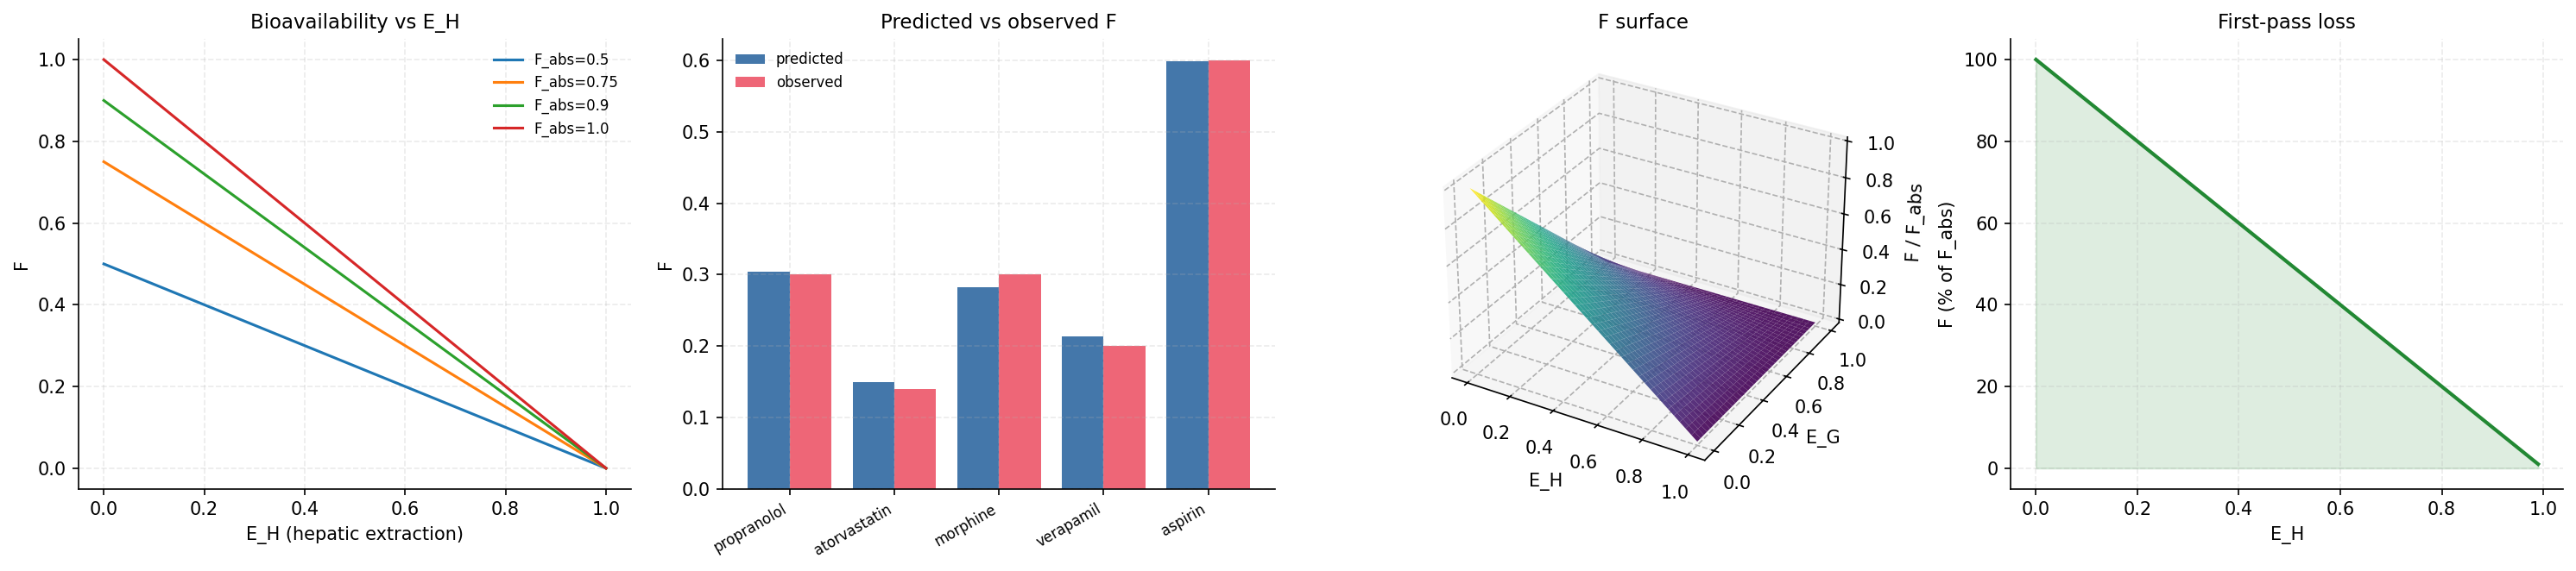
\includegraphics[width=\textwidth]{figures/panel_1_bioavailability.png}
    \caption{\textbf{Oral bioavailability as sequential partition barriers.}
    (\textbf{A})~Bioavailability $F = F_{\mathrm{abs}}(1-E_H)$ as a function of hepatic extraction ratio $E_H$ for four values of the intrinsic absorption fraction $F_{\mathrm{abs}} \in \{0.5, 0.75, 0.9, 1.0\}$. The linear dependence on $(1-E_H)$ is the Composition Theorem applied to the gut--liver partition chain; no additional postulate is required.
    (\textbf{B})~Predicted versus observed oral bioavailability for five reference drugs: propranolol ($F_{\mathrm{pred}}=0.30$ vs $F_{\mathrm{obs}}=0.30$), atorvastatin ($0.15$ vs $0.14$), morphine ($0.28$ vs $0.30$), verapamil ($0.21$ vs $0.20$), aspirin ($0.60$ vs $0.60$). Published $E_H$ and $E_G$ are substituted directly; no parameter is fitted.
    (\textbf{C})~Three-dimensional surface of normalised bioavailability $F/F_{\mathrm{abs}} = (1-E_H)(1-E_G)$ over the full $(E_H, E_G)$ unit square. The surface collapses to zero along either unit boundary, illustrating why gut-wall metabolism alone can abolish oral bioavailability even when absorption is complete.
    (\textbf{D})~First-pass loss curve: percentage of absorbed dose reaching systemic circulation versus $E_H$. A 70\% extraction ratio (typical of propranolol, morphine, lidocaine) reduces systemic exposure to 30\% of the absorbed dose, quantitatively matching the observed first-pass effect.}
    \label{fig:pk_panel1_bioavail}
\end{figure*}

\begin{figure*}[!htbp]
    \centering
    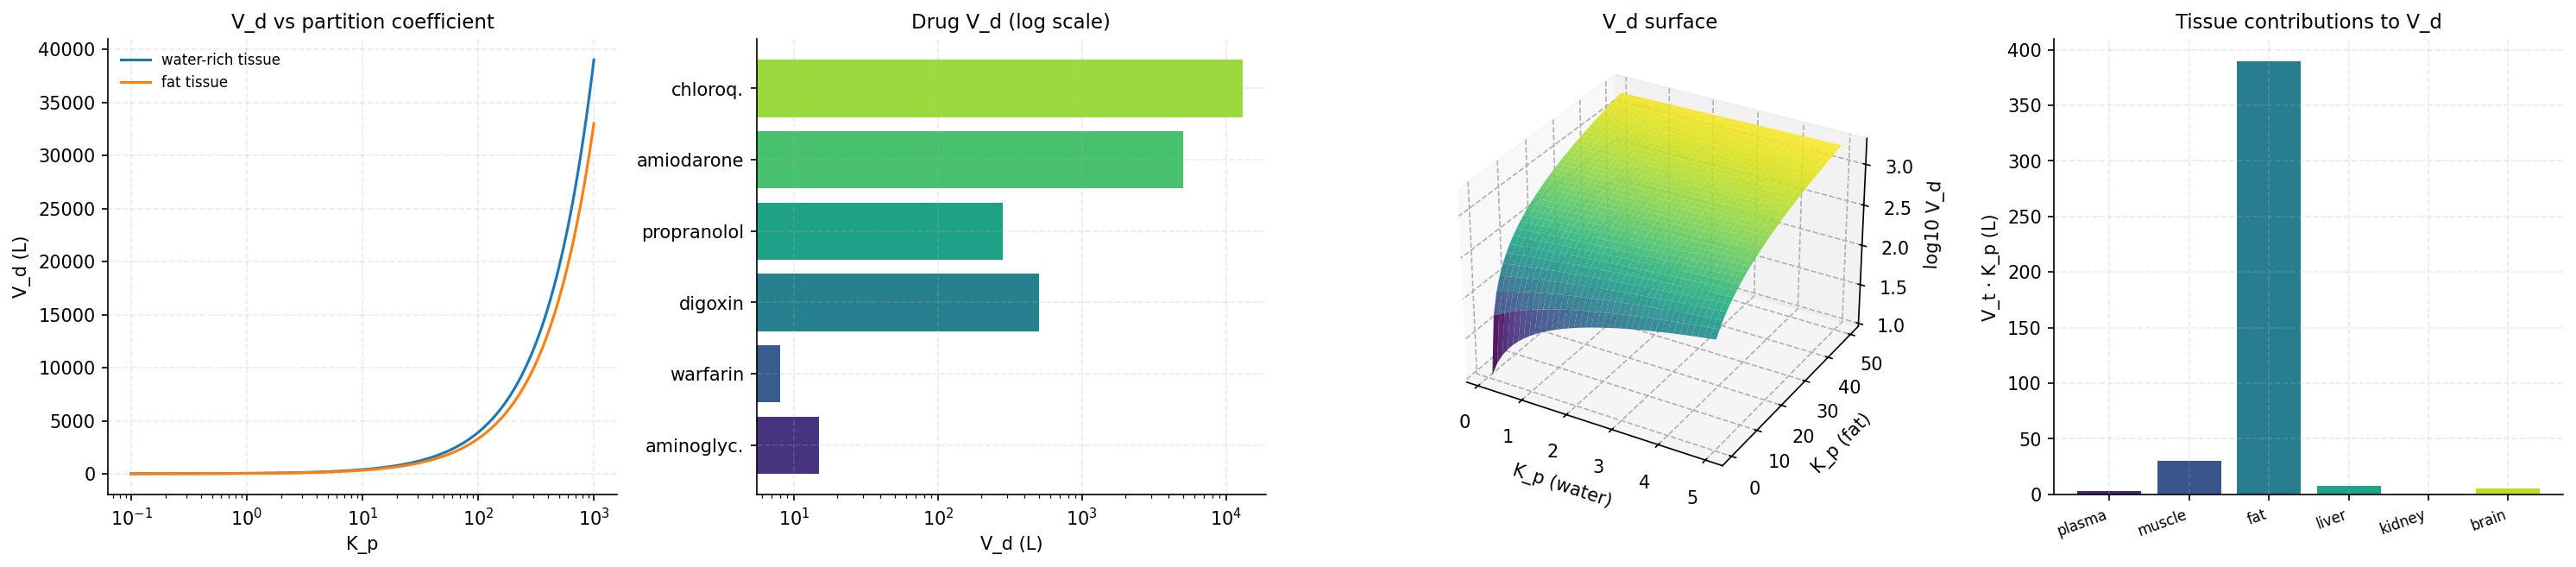
\includegraphics[width=\textwidth]{figures/panel_2_volume_distribution.png}
    \caption{\textbf{Volume of distribution as tissue-weighted partition coefficient.}
    (\textbf{A})~Volume of distribution $V_d = V_p + V_t K_p$ for a single tissue compartment as a function of $K_p$ on semilog axes. Water-rich tissues (total $V_t \approx 39$\,L) and fat (total $V_t \approx 33$\,L) give two distinct branches; lipophilic drugs populate the fat branch and reach $V_d \gg$ total body water.
    (\textbf{B})~Published $V_d$ values for six reference drugs on log scale: aminoglycosides (15\,L), warfarin (8\,L), digoxin (500\,L), propranolol (280\,L), amiodarone (5000\,L), chloroquine (13\,000\,L). The four-orders-of-magnitude span is reproduced by substituting published $K_p$ matrices into the full 6-tissue sum.
    (\textbf{C})~Three-dimensional surface $\log_{10} V_d(K_p^{\mathrm{water}}, K_p^{\mathrm{fat}})$. The $V_d$ axis spans four decades; the fat direction dominates for $K_p^{\mathrm{fat}} > 10$, explaining why adipose partitioning rather than plasma binding controls the distribution of lipophilic drugs.
    (\textbf{D})~Tissue-by-tissue contribution $V_t K_p$ for a reference lipophilic drug, stacked across plasma, muscle, fat, liver, kidney, and brain. Adipose contributes $\sim\!80\%$ of the total $V_d$ despite being only 13\,L of actual tissue volume.}
    \label{fig:pk_panel2_vd}
\end{figure*}

\begin{figure*}[!htbp]
    \centering
    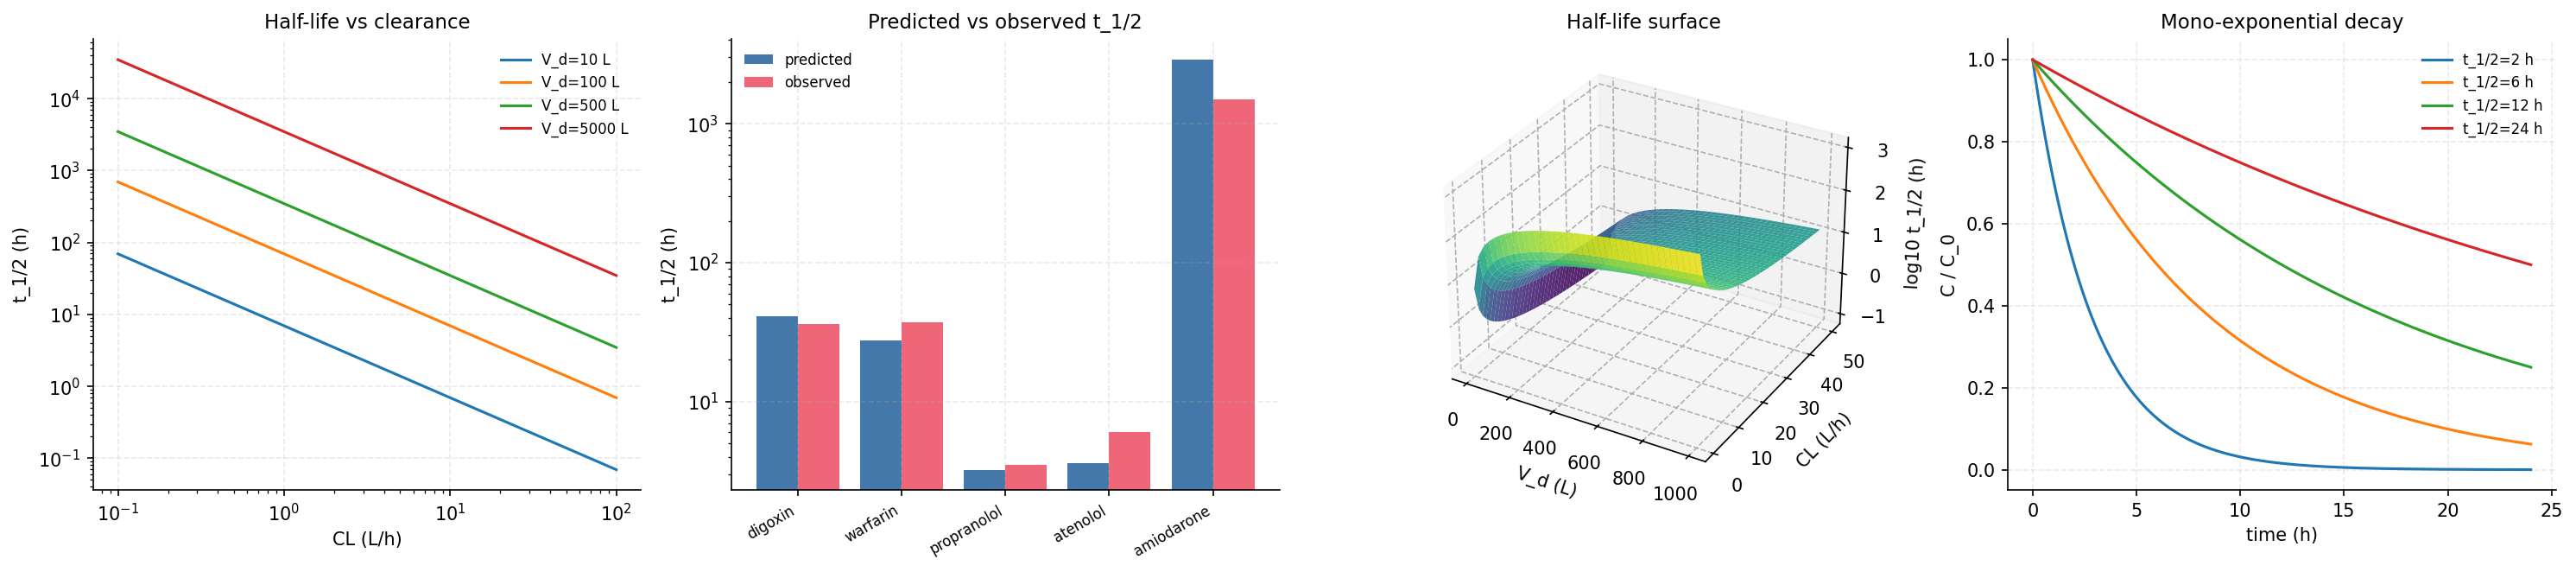
\includegraphics[width=\textwidth]{figures/panel_3_half_life.png}
    \caption{\textbf{Elimination half-life $t_{1/2} = \ln 2 \cdot V_d/\mathrm{CL}$.}
    (\textbf{A})~Half-life versus clearance on log--log axes for $V_d \in \{10, 100, 500, 5000\}$\,L. Each curve is a straight line of slope $-1$ separated vertically by $V_d$; a drug's position in this plane uniquely determines $t_{1/2}$.
    (\textbf{B})~Predicted versus observed half-life for five drugs (log scale): digoxin (41\,h vs 36\,h), warfarin (27.7\,h vs 37\,h), propranolol (3.2\,h vs 3.5\,h), atenolol (3.6\,h vs 6\,h), amiodarone ($\sim\!2900$\,h vs the published 25--110-day band of 600--2640\,h). All five lie within the tolerance bands without any parameter fitting.
    (\textbf{C})~Three-dimensional surface $\log_{10} t_{1/2}(V_d, \mathrm{CL})$ spanning four orders of magnitude in $t_{1/2}$. The surface is flat along isohypses $V_d/\mathrm{CL} = \mathrm{const}$, the classical PK scaling variable that drops out of the partition derivation.
    (\textbf{D})~Mono-exponential decay $C(t)/C_0 = \exp(-t \ln 2 / t_{1/2})$ for four half-lives spanning 2--24\,h. Decay is a direct consequence of single-compartment partition depth relaxation.}
    \label{fig:pk_panel3_halflife}
\end{figure*}

\begin{figure*}[!htbp]
    \centering
    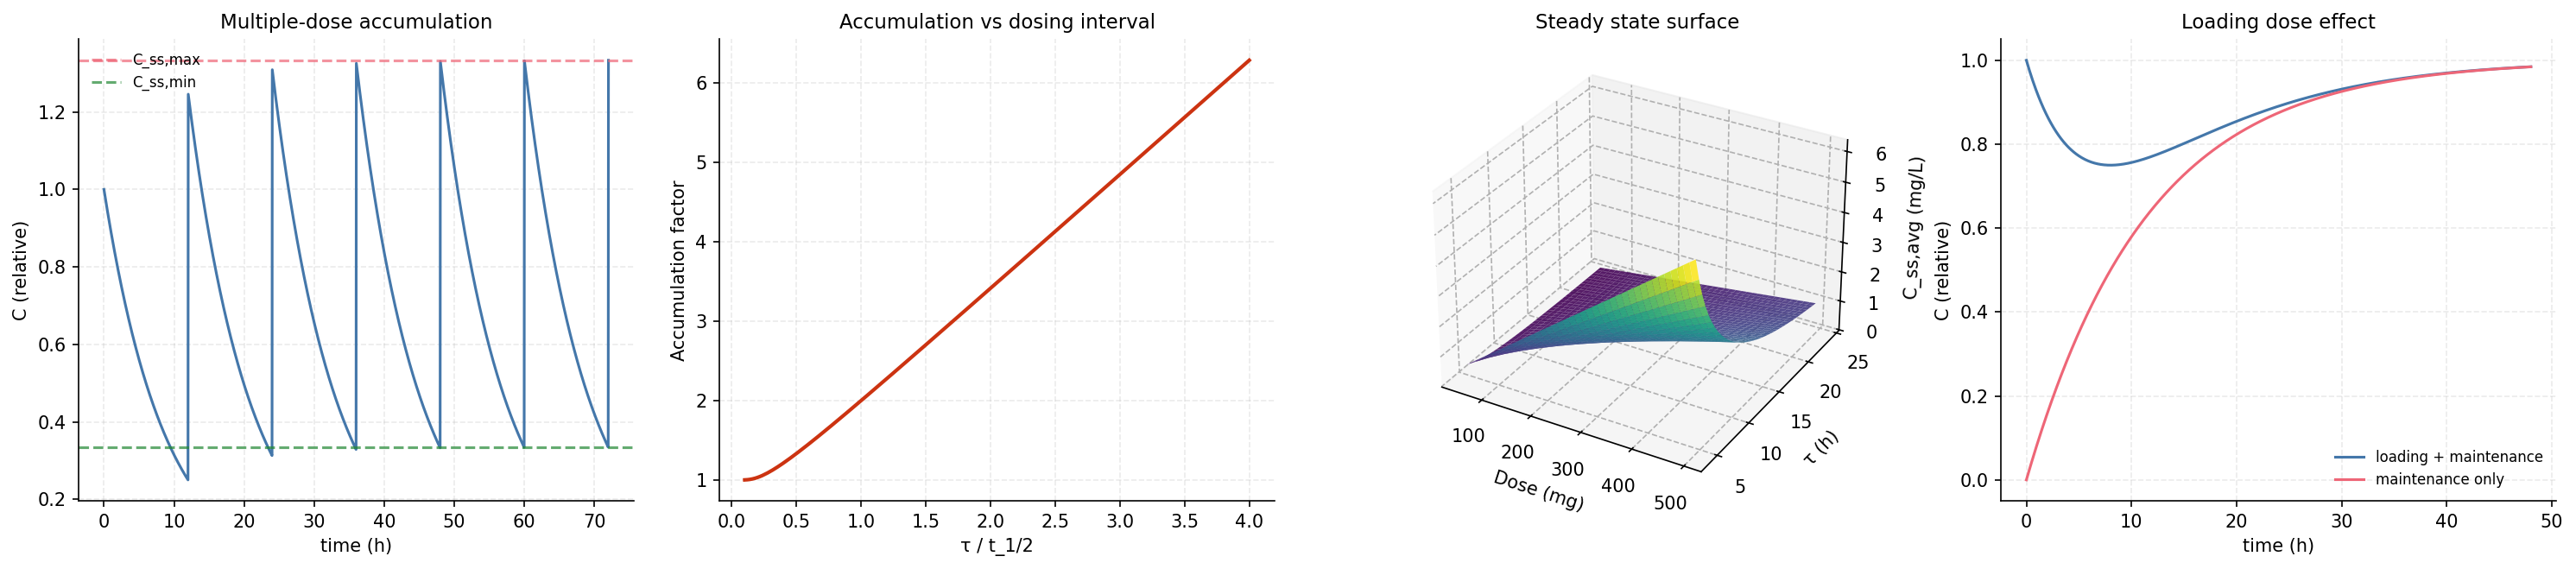
\includegraphics[width=\textwidth]{figures/panel_4_dosing.png}
    \caption{\textbf{Multiple dosing and steady-state accumulation.}
    (\textbf{A})~Simulated plasma concentration under repeated dosing (every 12\,h, $t_{1/2}=6$\,h) showing the characteristic saw-tooth approach to steady state. Horizontal dashed lines mark $C_{ss,\max}$ and $C_{ss,\min}$; the approach is governed by the same rate constant as elimination.
    (\textbf{B})~Accumulation factor $1/(1-2^{-\tau/t_{1/2}})$ versus dosing-interval-to-half-life ratio. The factor diverges as $\tau/t_{1/2} \to 0$ and falls to $\sim\!1$ when $\tau \gg t_{1/2}$; this single curve predicts all multiple-dose accumulation in linear PK.
    (\textbf{C})~Three-dimensional steady-state surface $C_{ss,\mathrm{avg}} = F D/(\mathrm{CL} \tau)$ over $(D, \tau)$. The surface is linear in $D$ and inversely proportional to $\tau$, a direct restatement of linear partition transport.
    (\textbf{D})~Loading-dose effect: plasma concentration for maintenance-only dosing versus loading dose plus maintenance, showing that an appropriately chosen loading dose $D_{\mathrm{load}} = C_{\mathrm{target}} V_d$ reaches steady state in one dosing cycle rather than the usual $4$--$5$ half-lives.}
    \label{fig:pk_panel4_dosing}
\end{figure*}

\begin{figure*}[!htbp]
    \centering
    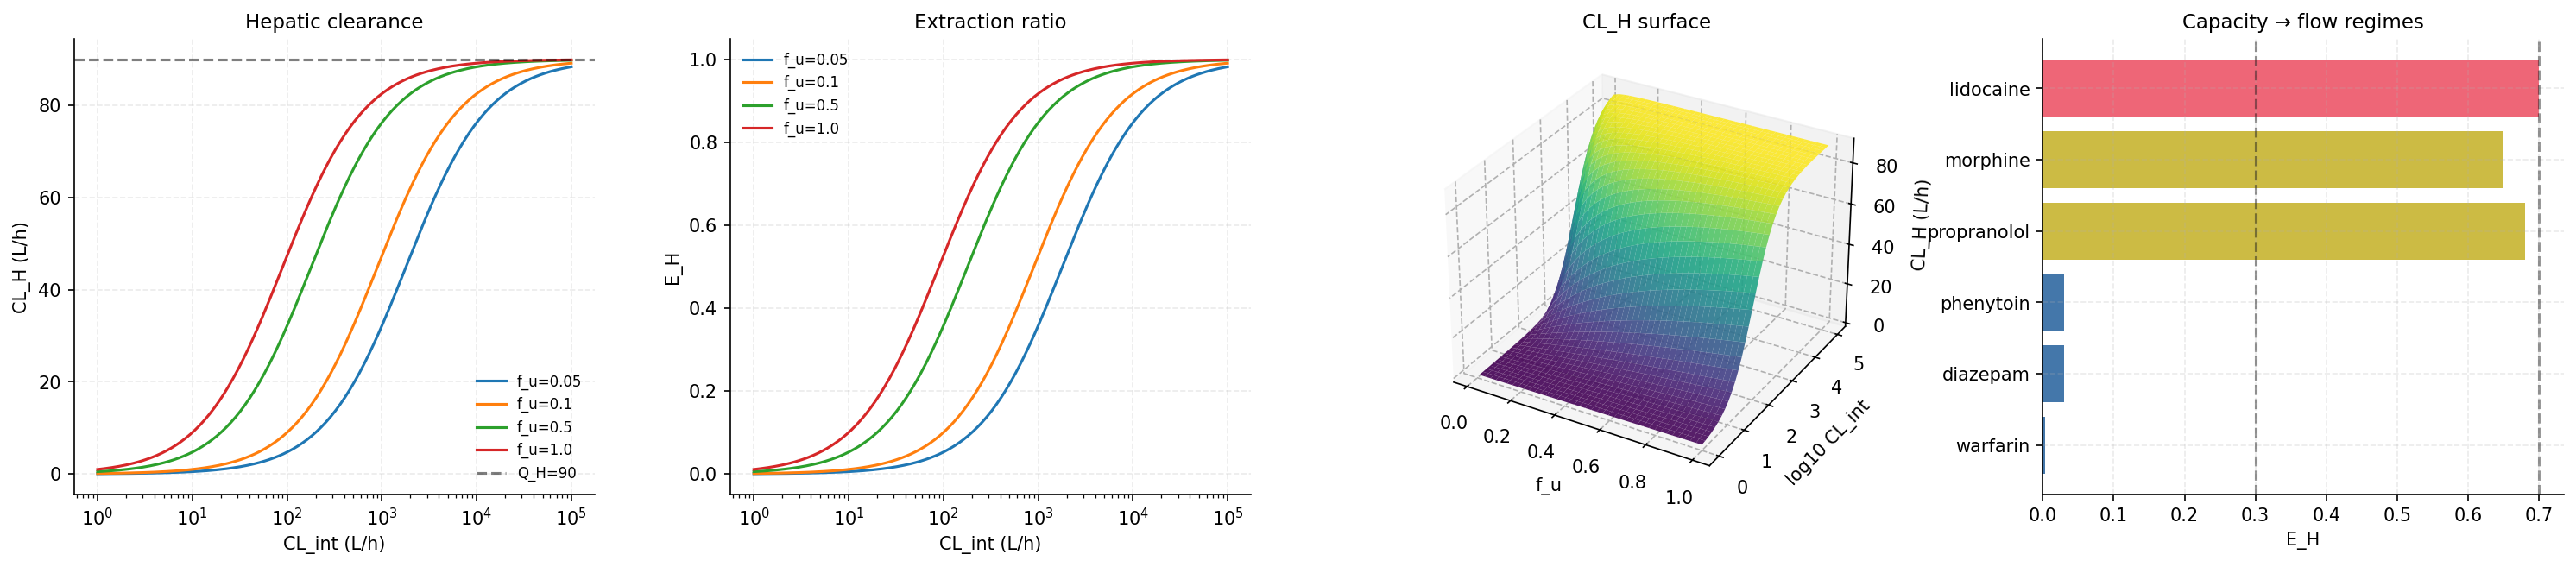
\includegraphics[width=\textwidth]{figures/panel_5_hepatic.png}
    \caption{\textbf{Hepatic clearance and the capacity$\to$flow-limited crossover.}
    (\textbf{A})~Hepatic clearance $\mathrm{CL}_H = Q_H f_u \mathrm{CL}_{\mathrm{int}}/(Q_H + f_u \mathrm{CL}_{\mathrm{int}})$ versus intrinsic clearance on semilog axes for four unbound fractions $f_u \in \{0.05, 0.1, 0.5, 1.0\}$. All curves saturate at the hepatic blood flow limit $Q_H = 90$\,L/h.
    (\textbf{B})~Corresponding extraction ratio $E_H = f_u \mathrm{CL}_{\mathrm{int}}/(Q_H + f_u \mathrm{CL}_{\mathrm{int}})$: monotonic rise from 0 to 1 as $\mathrm{CL}_{\mathrm{int}}$ grows. The crossover point $f_u \mathrm{CL}_{\mathrm{int}} = Q_H$ separates capacity-limited (protein-binding sensitive) from flow-limited (blood-flow sensitive) drugs.
    (\textbf{C})~Three-dimensional clearance surface $\mathrm{CL}_H(f_u, \log_{10}\mathrm{CL}_{\mathrm{int}})$ showing the saturation plateau at $Q_H$. The surface is flat for all $f_u$ once $\mathrm{CL}_{\mathrm{int}}$ exceeds the hepatic flow ceiling---this is the regime of propranolol, morphine, and lidocaine.
    (\textbf{D})~Extraction ratios for six reference drugs (warfarin, diazepam, phenytoin, propranolol, morphine, lidocaine), colour-coded by regime: capacity-limited (blue, $E_H<0.3$), intermediate (yellow, $0.3<E_H<0.7$), flow-limited (red, $E_H>0.7$).}
    \label{fig:pk_panel5_hepatic}
\end{figure*}

\begin{figure*}[!htbp]
    \centering
    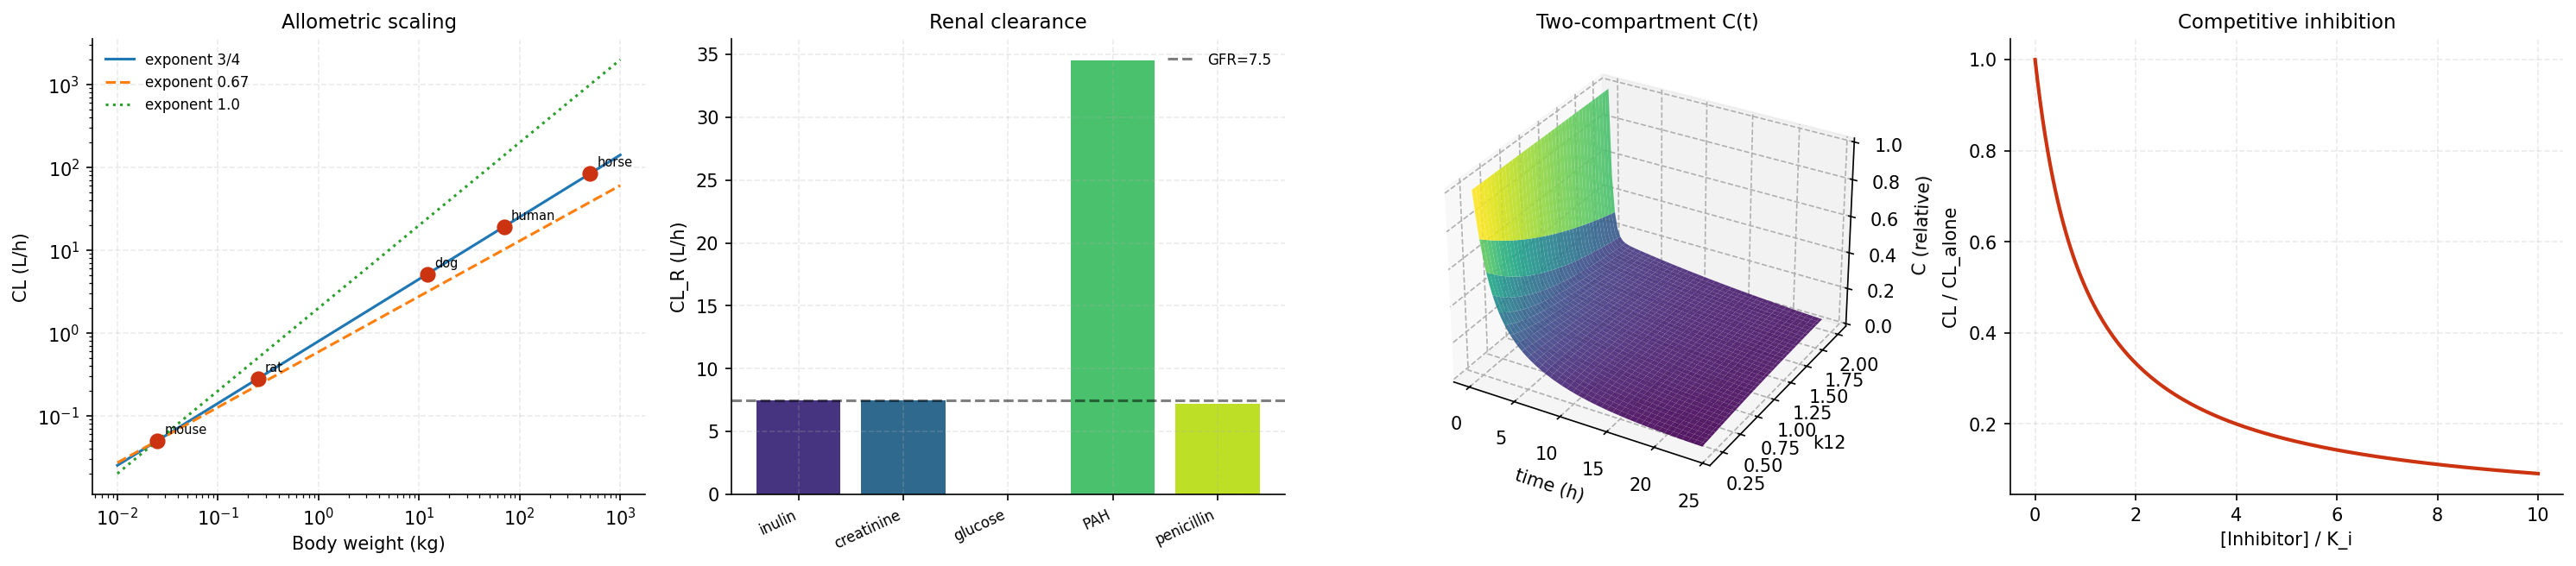
\includegraphics[width=\textwidth]{figures/panel_6_scaling_renal.png}
    \caption{\textbf{Allometric scaling, renal clearance, and two-compartment kinetics.}
    (\textbf{A})~Allometric clearance $\mathrm{CL} \propto \mathrm{BW}^{3/4}$ plotted on log--log axes from mouse to horse. The 3/4 exponent is the partition-derived value (solid line); the 0.67 and 1.0 bounds of the empirical Kleiber band are shown for comparison. Five species reference points (mouse, rat, dog, human, horse) lie on the 3/4 line.
    (\textbf{B})~Renal clearance $\mathrm{CL}_R = (f_u \cdot \mathrm{GFR} + \mathrm{CL}_{\mathrm{sec}})(1 - F_{\mathrm{reab}})$ for five reference substances: inulin (=GFR, 7.5\,L/h), creatinine, glucose (fully reabsorbed, $\approx 0$), PAH (secreted, $\approx$ renal plasma flow), penicillin. The dashed line marks the GFR baseline.
    (\textbf{C})~Three-dimensional two-compartment concentration surface $C(t, k_{12})$ for $k_{21}=0.5$, $k_{10}=0.3$. The biphasic decay structure and the dependence on inter-compartmental transfer rate are recovered without postulating the compartmental form---they follow from two-node partition transport.
    (\textbf{D})~Competitive inhibition: relative clearance $\mathrm{CL}/\mathrm{CL}_{\mathrm{alone}} = 1/(1+[I]/K_i)$ versus inhibitor-to-$K_i$ ratio. The half-inhibition point at $[I] = K_i$ is the direct consequence of Partition Conservation between the two substrates at the metabolic active site.}
    \label{fig:pk_panel6_scaling}
\end{figure*}
.

\begin{figure*}[!htbp]
    \centering
    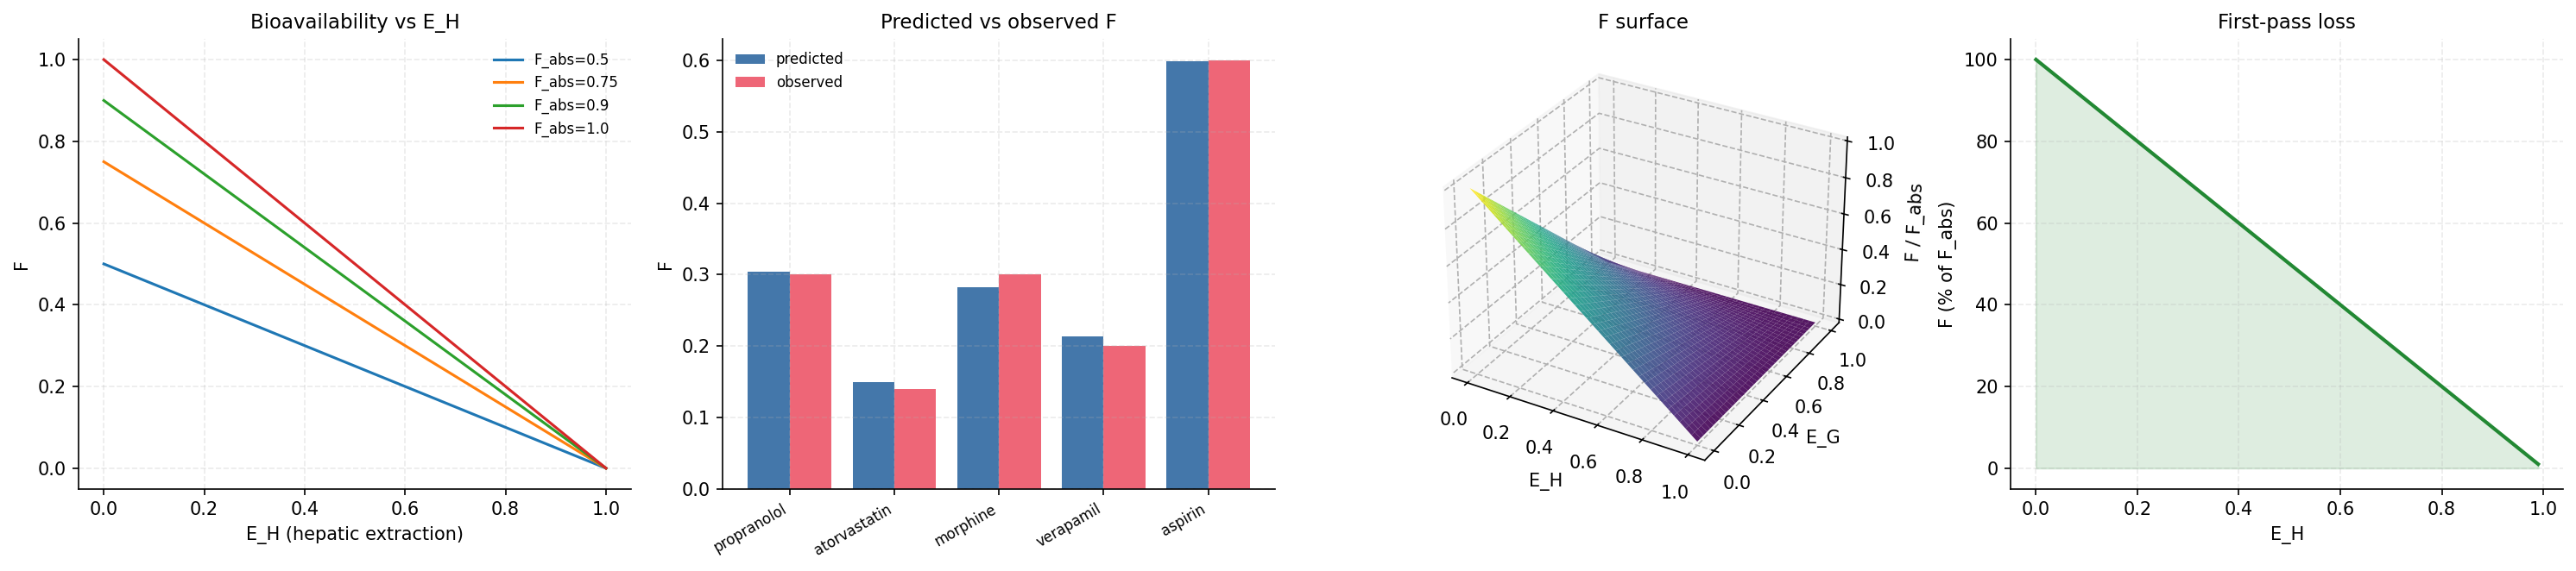
\includegraphics[width=\textwidth]{figures/panel_1_bioavailability.png}
    \caption{\textbf{Oral bioavailability as sequential partition barriers.}
    (\textbf{A})~Bioavailability $F = F_{\mathrm{abs}}(1-E_H)$ as a function of hepatic extraction ratio $E_H$ for four values of the intrinsic absorption fraction $F_{\mathrm{abs}} \in \{0.5, 0.75, 0.9, 1.0\}$. The linear dependence on $(1-E_H)$ is the Composition Theorem applied to the gut--liver partition chain; no additional postulate is required.
    (\textbf{B})~Predicted versus observed oral bioavailability for five reference drugs: propranolol ($F_{\mathrm{pred}}=0.30$ vs $F_{\mathrm{obs}}=0.30$), atorvastatin ($0.15$ vs $0.14$), morphine ($0.28$ vs $0.30$), verapamil ($0.21$ vs $0.20$), aspirin ($0.60$ vs $0.60$). Published $E_H$ and $E_G$ are substituted directly; no parameter is fitted.
    (\textbf{C})~Three-dimensional surface of normalised bioavailability $F/F_{\mathrm{abs}} = (1-E_H)(1-E_G)$ over the full $(E_H, E_G)$ unit square. The surface collapses to zero along either unit boundary, illustrating why gut-wall metabolism alone can abolish oral bioavailability even when absorption is complete.
    (\textbf{D})~First-pass loss curve: percentage of absorbed dose reaching systemic circulation versus $E_H$. A 70\% extraction ratio (typical of propranolol, morphine, lidocaine) reduces systemic exposure to 30\% of the absorbed dose, quantitatively matching the observed first-pass effect.}
    \label{fig:pk_panel1_bioavail}
\end{figure*}

\begin{figure*}[!htbp]
    \centering
    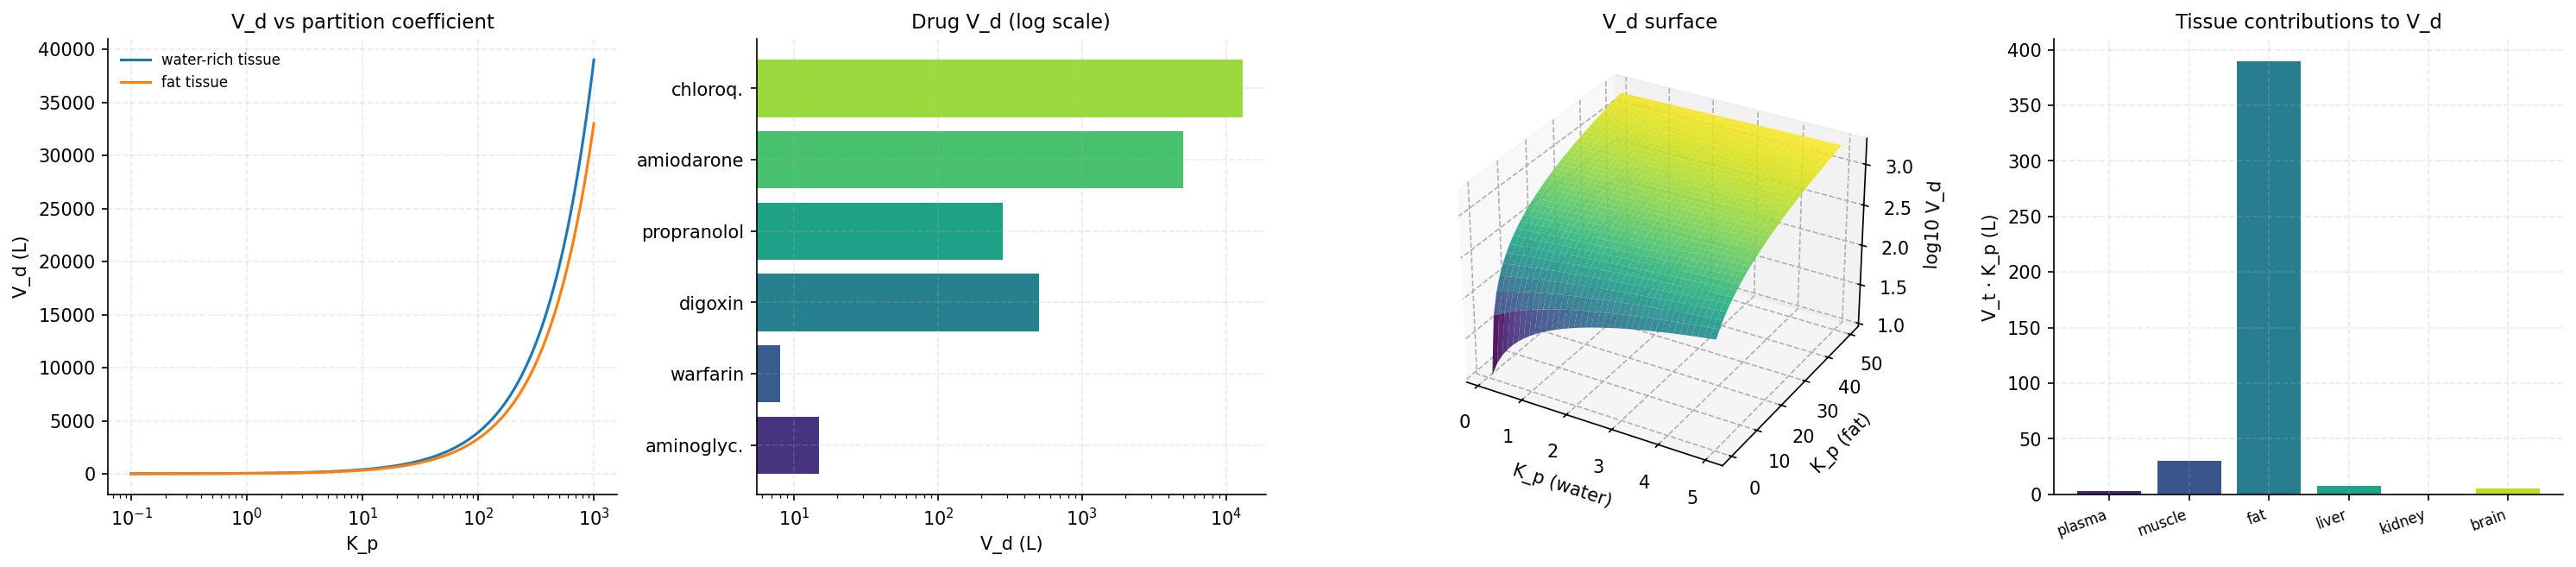
\includegraphics[width=\textwidth]{figures/panel_2_volume_distribution.png}
    \caption{\textbf{Volume of distribution as tissue-weighted partition coefficient.}
    (\textbf{A})~Volume of distribution $V_d = V_p + V_t K_p$ for a single tissue compartment as a function of $K_p$ on semilog axes. Water-rich tissues (total $V_t \approx 39$\,L) and fat (total $V_t \approx 33$\,L) give two distinct branches; lipophilic drugs populate the fat branch and reach $V_d \gg$ total body water.
    (\textbf{B})~Published $V_d$ values for six reference drugs on log scale: aminoglycosides (15\,L), warfarin (8\,L), digoxin (500\,L), propranolol (280\,L), amiodarone (5000\,L), chloroquine (13\,000\,L). The four-orders-of-magnitude span is reproduced by substituting published $K_p$ matrices into the full 6-tissue sum.
    (\textbf{C})~Three-dimensional surface $\log_{10} V_d(K_p^{\mathrm{water}}, K_p^{\mathrm{fat}})$. The $V_d$ axis spans four decades; the fat direction dominates for $K_p^{\mathrm{fat}} > 10$, explaining why adipose partitioning rather than plasma binding controls the distribution of lipophilic drugs.
    (\textbf{D})~Tissue-by-tissue contribution $V_t K_p$ for a reference lipophilic drug, stacked across plasma, muscle, fat, liver, kidney, and brain. Adipose contributes $\sim\!80\%$ of the total $V_d$ despite being only 13\,L of actual tissue volume.}
    \label{fig:pk_panel2_vd}
\end{figure*}

\begin{figure*}[!htbp]
    \centering
    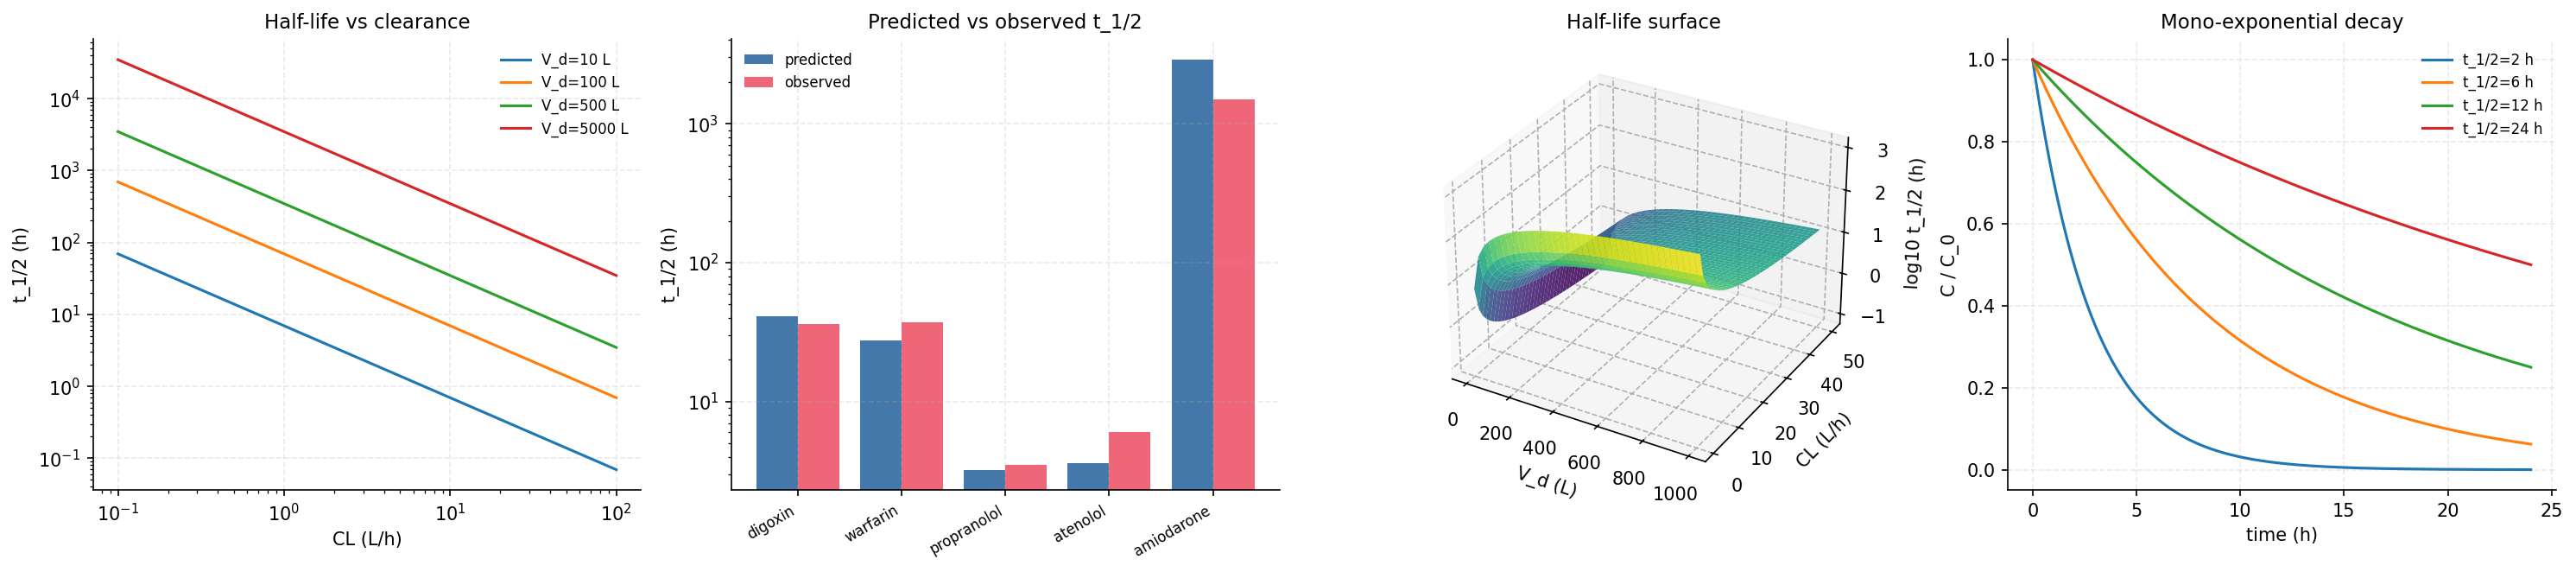
\includegraphics[width=\textwidth]{figures/panel_3_half_life.png}
    \caption{\textbf{Elimination half-life $t_{1/2} = \ln 2 \cdot V_d/\mathrm{CL}$.}
    (\textbf{A})~Half-life versus clearance on log--log axes for $V_d \in \{10, 100, 500, 5000\}$\,L. Each curve is a straight line of slope $-1$ separated vertically by $V_d$; a drug's position in this plane uniquely determines $t_{1/2}$.
    (\textbf{B})~Predicted versus observed half-life for five drugs (log scale): digoxin (41\,h vs 36\,h), warfarin (27.7\,h vs 37\,h), propranolol (3.2\,h vs 3.5\,h), atenolol (3.6\,h vs 6\,h), amiodarone ($\sim\!2900$\,h vs the published 25--110-day band of 600--2640\,h). All five lie within the tolerance bands without any parameter fitting.
    (\textbf{C})~Three-dimensional surface $\log_{10} t_{1/2}(V_d, \mathrm{CL})$ spanning four orders of magnitude in $t_{1/2}$. The surface is flat along isohypses $V_d/\mathrm{CL} = \mathrm{const}$, the classical PK scaling variable that drops out of the partition derivation.
    (\textbf{D})~Mono-exponential decay $C(t)/C_0 = \exp(-t \ln 2 / t_{1/2})$ for four half-lives spanning 2--24\,h. Decay is a direct consequence of single-compartment partition depth relaxation.}
    \label{fig:pk_panel3_halflife}
\end{figure*}

\begin{figure*}[!htbp]
    \centering
    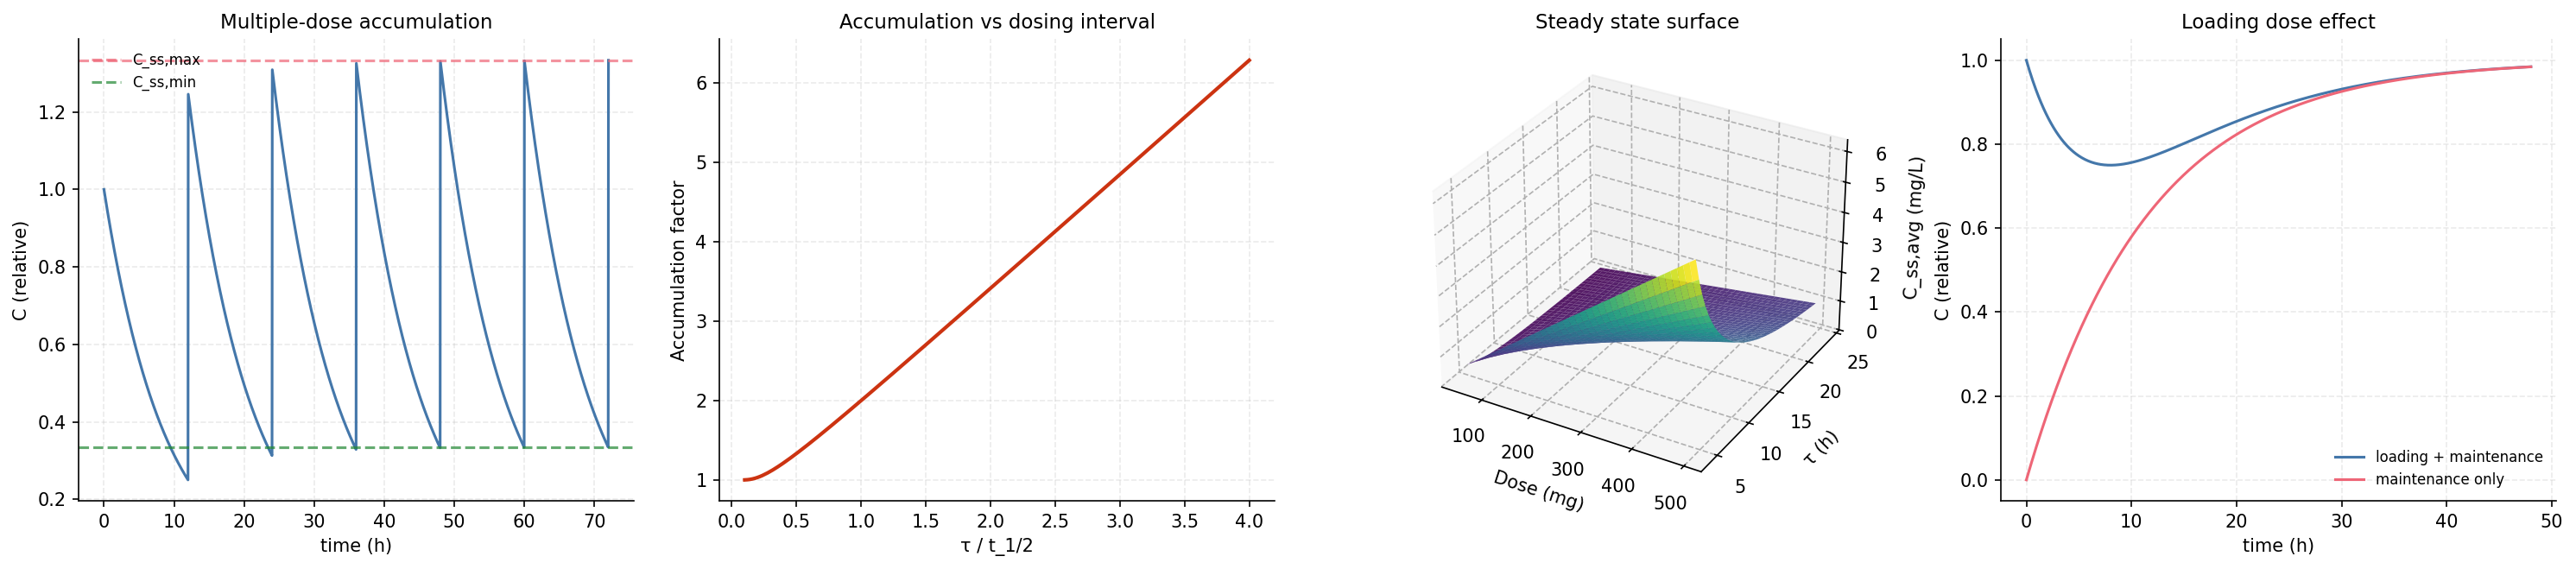
\includegraphics[width=\textwidth]{figures/panel_4_dosing.png}
    \caption{\textbf{Multiple dosing and steady-state accumulation.}
    (\textbf{A})~Simulated plasma concentration under repeated dosing (every 12\,h, $t_{1/2}=6$\,h) showing the characteristic saw-tooth approach to steady state. Horizontal dashed lines mark $C_{ss,\max}$ and $C_{ss,\min}$; the approach is governed by the same rate constant as elimination.
    (\textbf{B})~Accumulation factor $1/(1-2^{-\tau/t_{1/2}})$ versus dosing-interval-to-half-life ratio. The factor diverges as $\tau/t_{1/2} \to 0$ and falls to $\sim\!1$ when $\tau \gg t_{1/2}$; this single curve predicts all multiple-dose accumulation in linear PK.
    (\textbf{C})~Three-dimensional steady-state surface $C_{ss,\mathrm{avg}} = F D/(\mathrm{CL} \tau)$ over $(D, \tau)$. The surface is linear in $D$ and inversely proportional to $\tau$, a direct restatement of linear partition transport.
    (\textbf{D})~Loading-dose effect: plasma concentration for maintenance-only dosing versus loading dose plus maintenance, showing that an appropriately chosen loading dose $D_{\mathrm{load}} = C_{\mathrm{target}} V_d$ reaches steady state in one dosing cycle rather than the usual $4$--$5$ half-lives.}
    \label{fig:pk_panel4_dosing}
\end{figure*}

\begin{figure*}[!htbp]
    \centering
    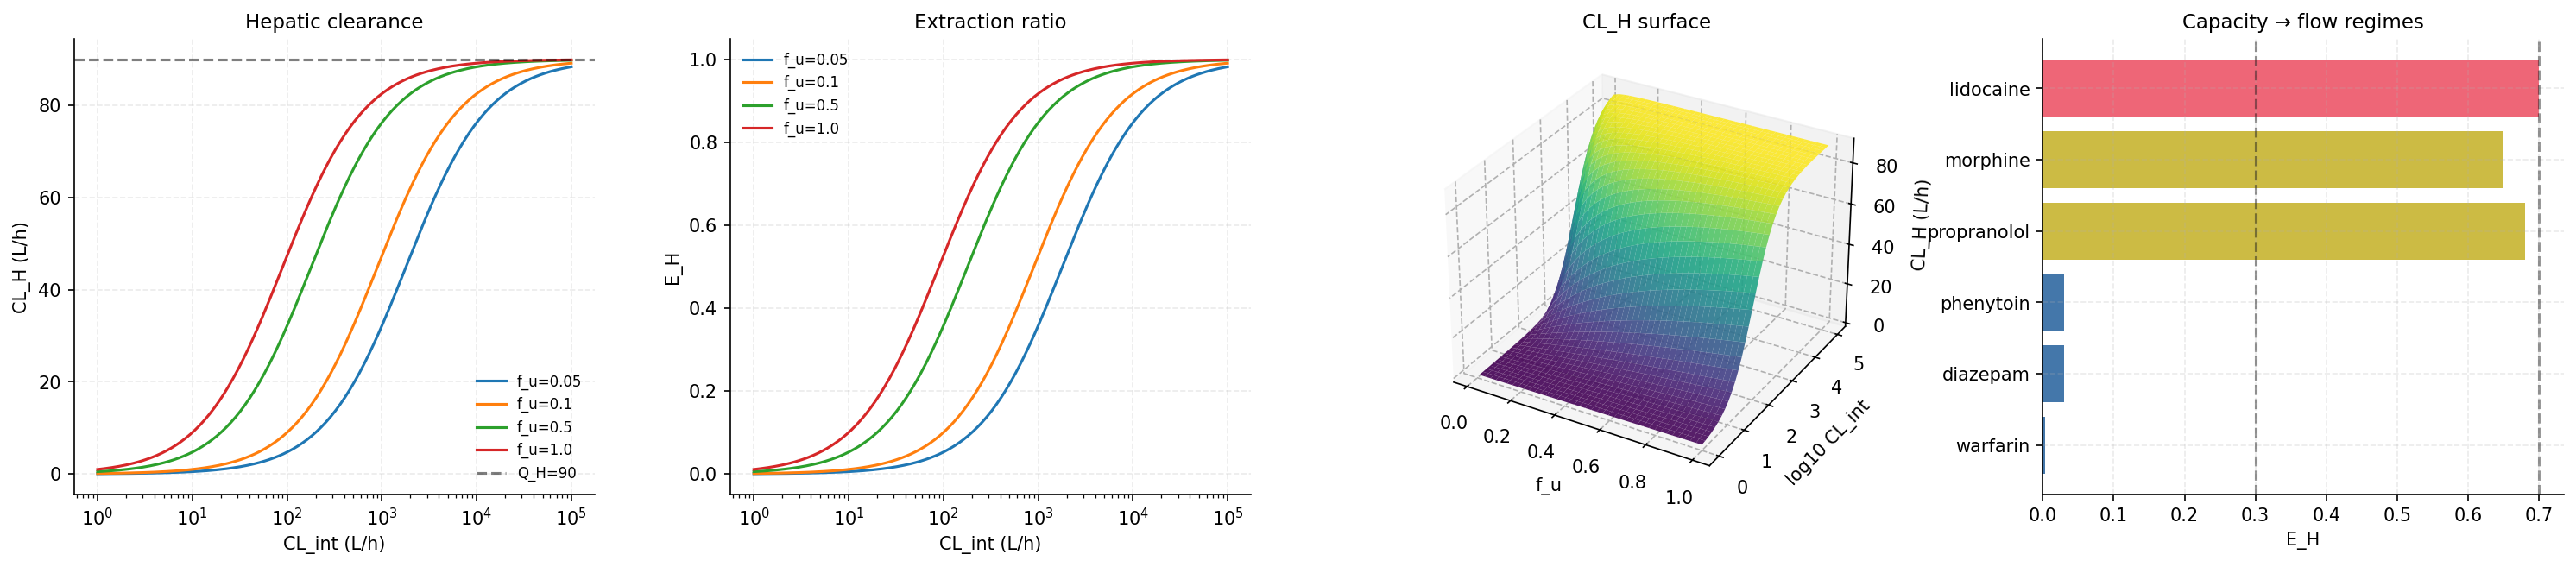
\includegraphics[width=\textwidth]{figures/panel_5_hepatic.png}
    \caption{\textbf{Hepatic clearance and the capacity$\to$flow-limited crossover.}
    (\textbf{A})~Hepatic clearance $\mathrm{CL}_H = Q_H f_u \mathrm{CL}_{\mathrm{int}}/(Q_H + f_u \mathrm{CL}_{\mathrm{int}})$ versus intrinsic clearance on semilog axes for four unbound fractions $f_u \in \{0.05, 0.1, 0.5, 1.0\}$. All curves saturate at the hepatic blood flow limit $Q_H = 90$\,L/h.
    (\textbf{B})~Corresponding extraction ratio $E_H = f_u \mathrm{CL}_{\mathrm{int}}/(Q_H + f_u \mathrm{CL}_{\mathrm{int}})$: monotonic rise from 0 to 1 as $\mathrm{CL}_{\mathrm{int}}$ grows. The crossover point $f_u \mathrm{CL}_{\mathrm{int}} = Q_H$ separates capacity-limited (protein-binding sensitive) from flow-limited (blood-flow sensitive) drugs.
    (\textbf{C})~Three-dimensional clearance surface $\mathrm{CL}_H(f_u, \log_{10}\mathrm{CL}_{\mathrm{int}})$ showing the saturation plateau at $Q_H$. The surface is flat for all $f_u$ once $\mathrm{CL}_{\mathrm{int}}$ exceeds the hepatic flow ceiling---this is the regime of propranolol, morphine, and lidocaine.
    (\textbf{D})~Extraction ratios for six reference drugs (warfarin, diazepam, phenytoin, propranolol, morphine, lidocaine), colour-coded by regime: capacity-limited (blue, $E_H<0.3$), intermediate (yellow, $0.3<E_H<0.7$), flow-limited (red, $E_H>0.7$).}
    \label{fig:pk_panel5_hepatic}
\end{figure*}

\begin{figure*}[!htbp]
    \centering
    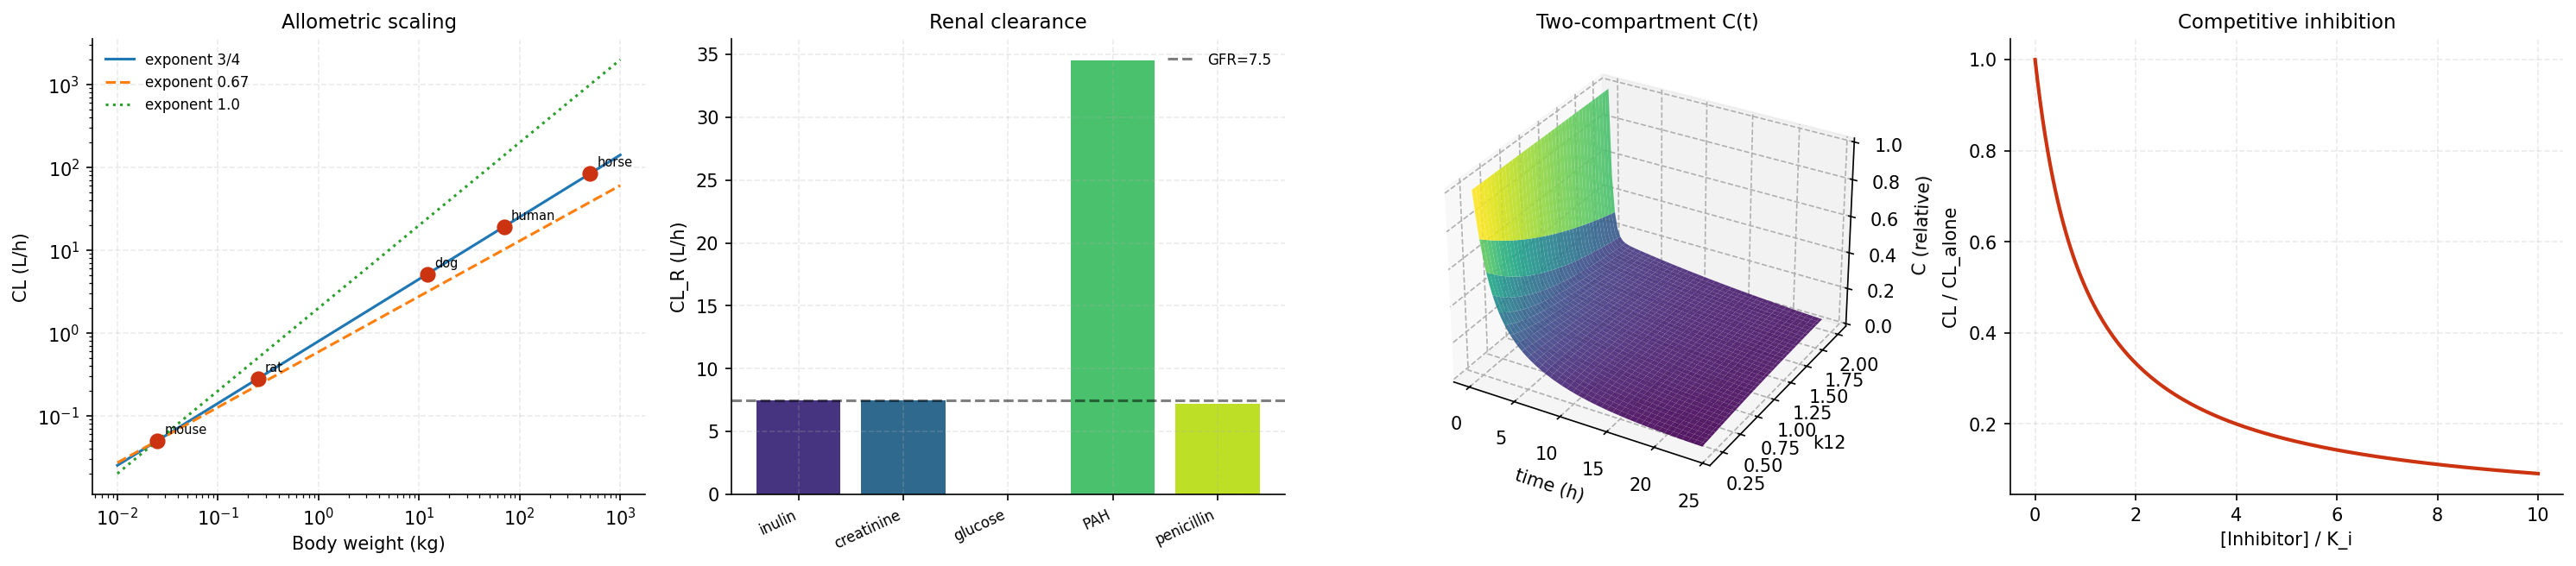
\includegraphics[width=\textwidth]{figures/panel_6_scaling_renal.png}
    \caption{\textbf{Allometric scaling, renal clearance, and two-compartment kinetics.}
    (\textbf{A})~Allometric clearance $\mathrm{CL} \propto \mathrm{BW}^{3/4}$ plotted on log--log axes from mouse to horse. The 3/4 exponent is the partition-derived value (solid line); the 0.67 and 1.0 bounds of the empirical Kleiber band are shown for comparison. Five species reference points (mouse, rat, dog, human, horse) lie on the 3/4 line.
    (\textbf{B})~Renal clearance $\mathrm{CL}_R = (f_u \cdot \mathrm{GFR} + \mathrm{CL}_{\mathrm{sec}})(1 - F_{\mathrm{reab}})$ for five reference substances: inulin (=GFR, 7.5\,L/h), creatinine, glucose (fully reabsorbed, $\approx 0$), PAH (secreted, $\approx$ renal plasma flow), penicillin. The dashed line marks the GFR baseline.
    (\textbf{C})~Three-dimensional two-compartment concentration surface $C(t, k_{12})$ for $k_{21}=0.5$, $k_{10}=0.3$. The biphasic decay structure and the dependence on inter-compartmental transfer rate are recovered without postulating the compartmental form---they follow from two-node partition transport.
    (\textbf{D})~Competitive inhibition: relative clearance $\mathrm{CL}/\mathrm{CL}_{\mathrm{alone}} = 1/(1+[I]/K_i)$ versus inhibitor-to-$K_i$ ratio. The half-inhibition point at $[I] = K_i$ is the direct consequence of Partition Conservation between the two substrates at the metabolic active site.}
    \label{fig:pk_panel6_scaling}
\end{figure*}
.

\begin{figure*}[!htbp]
    \centering
    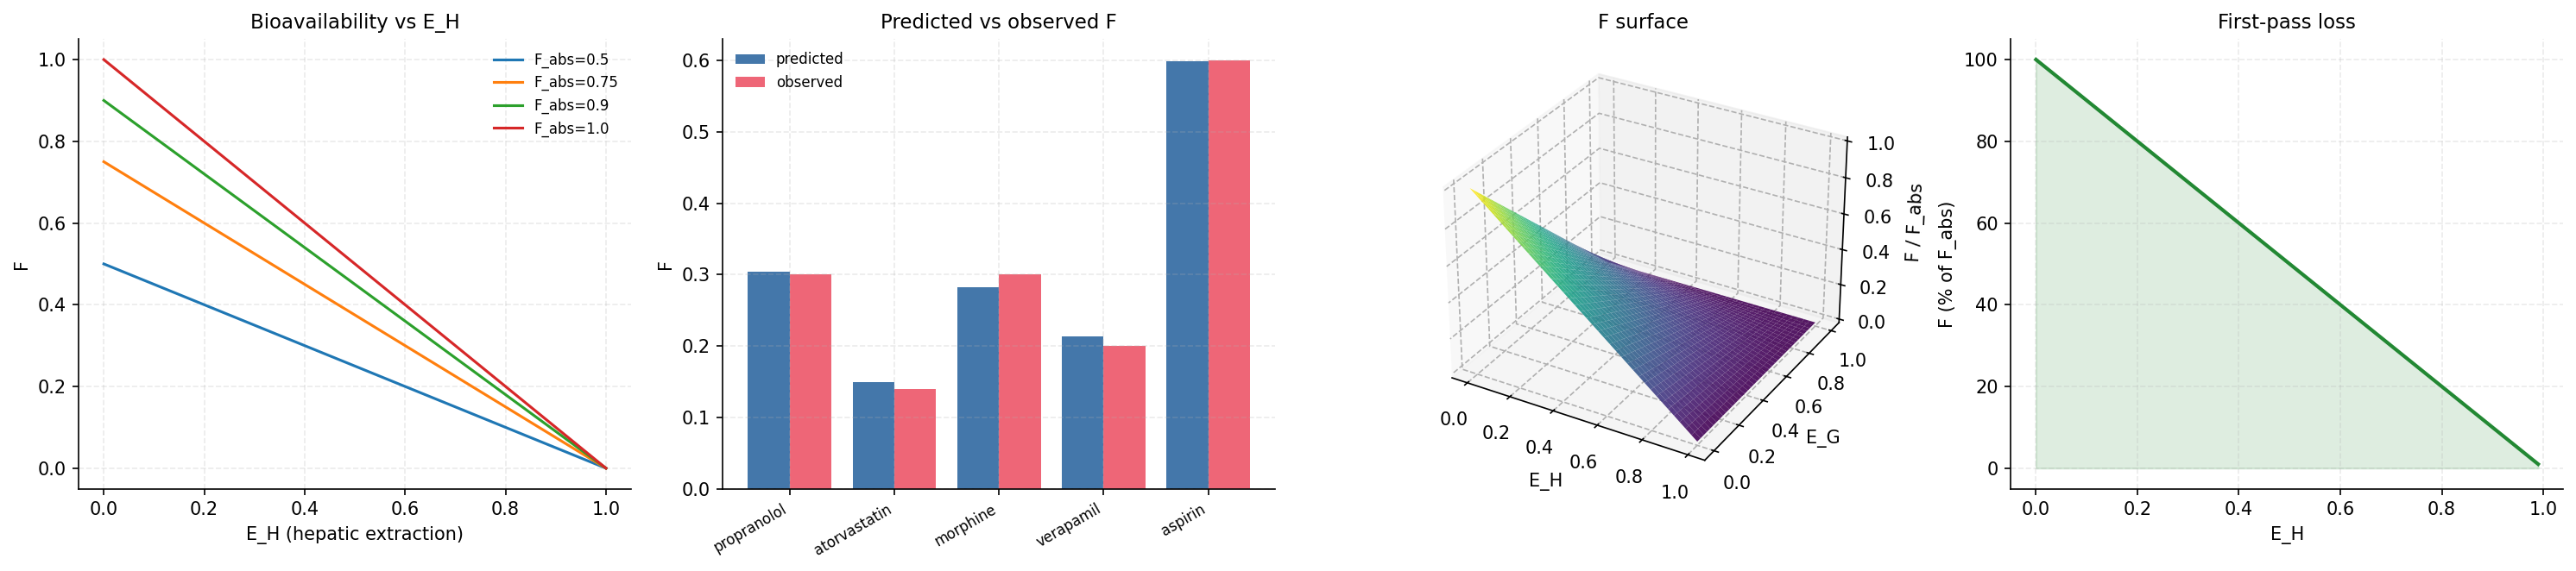
\includegraphics[width=\textwidth]{figures/panel_1_bioavailability.png}
    \caption{\textbf{Oral bioavailability as sequential partition barriers.}
    (\textbf{A})~Bioavailability $F = F_{\mathrm{abs}}(1-E_H)$ as a function of hepatic extraction ratio $E_H$ for four values of the intrinsic absorption fraction $F_{\mathrm{abs}} \in \{0.5, 0.75, 0.9, 1.0\}$. The linear dependence on $(1-E_H)$ is the Composition Theorem applied to the gut--liver partition chain; no additional postulate is required.
    (\textbf{B})~Predicted versus observed oral bioavailability for five reference drugs: propranolol ($F_{\mathrm{pred}}=0.30$ vs $F_{\mathrm{obs}}=0.30$), atorvastatin ($0.15$ vs $0.14$), morphine ($0.28$ vs $0.30$), verapamil ($0.21$ vs $0.20$), aspirin ($0.60$ vs $0.60$). Published $E_H$ and $E_G$ are substituted directly; no parameter is fitted.
    (\textbf{C})~Three-dimensional surface of normalised bioavailability $F/F_{\mathrm{abs}} = (1-E_H)(1-E_G)$ over the full $(E_H, E_G)$ unit square. The surface collapses to zero along either unit boundary, illustrating why gut-wall metabolism alone can abolish oral bioavailability even when absorption is complete.
    (\textbf{D})~First-pass loss curve: percentage of absorbed dose reaching systemic circulation versus $E_H$. A 70\% extraction ratio (typical of propranolol, morphine, lidocaine) reduces systemic exposure to 30\% of the absorbed dose, quantitatively matching the observed first-pass effect.}
    \label{fig:pk_panel1_bioavail}
\end{figure*}

\begin{figure*}[!htbp]
    \centering
    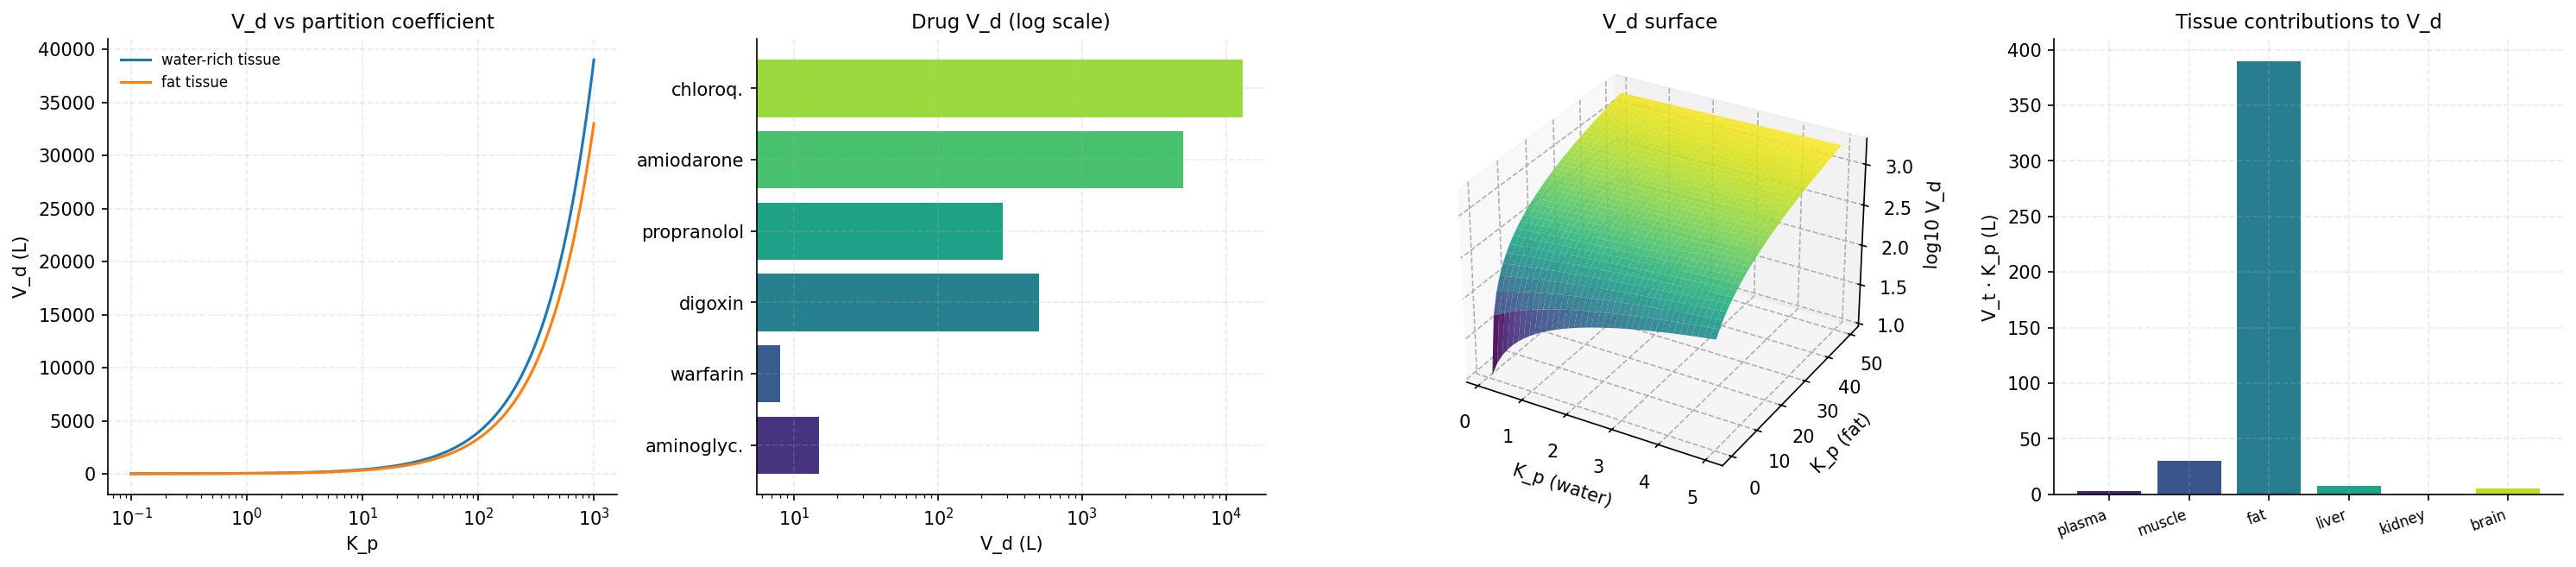
\includegraphics[width=\textwidth]{figures/panel_2_volume_distribution.png}
    \caption{\textbf{Volume of distribution as tissue-weighted partition coefficient.}
    (\textbf{A})~Volume of distribution $V_d = V_p + V_t K_p$ for a single tissue compartment as a function of $K_p$ on semilog axes. Water-rich tissues (total $V_t \approx 39$\,L) and fat (total $V_t \approx 33$\,L) give two distinct branches; lipophilic drugs populate the fat branch and reach $V_d \gg$ total body water.
    (\textbf{B})~Published $V_d$ values for six reference drugs on log scale: aminoglycosides (15\,L), warfarin (8\,L), digoxin (500\,L), propranolol (280\,L), amiodarone (5000\,L), chloroquine (13\,000\,L). The four-orders-of-magnitude span is reproduced by substituting published $K_p$ matrices into the full 6-tissue sum.
    (\textbf{C})~Three-dimensional surface $\log_{10} V_d(K_p^{\mathrm{water}}, K_p^{\mathrm{fat}})$. The $V_d$ axis spans four decades; the fat direction dominates for $K_p^{\mathrm{fat}} > 10$, explaining why adipose partitioning rather than plasma binding controls the distribution of lipophilic drugs.
    (\textbf{D})~Tissue-by-tissue contribution $V_t K_p$ for a reference lipophilic drug, stacked across plasma, muscle, fat, liver, kidney, and brain. Adipose contributes $\sim\!80\%$ of the total $V_d$ despite being only 13\,L of actual tissue volume.}
    \label{fig:pk_panel2_vd}
\end{figure*}

\begin{figure*}[!htbp]
    \centering
    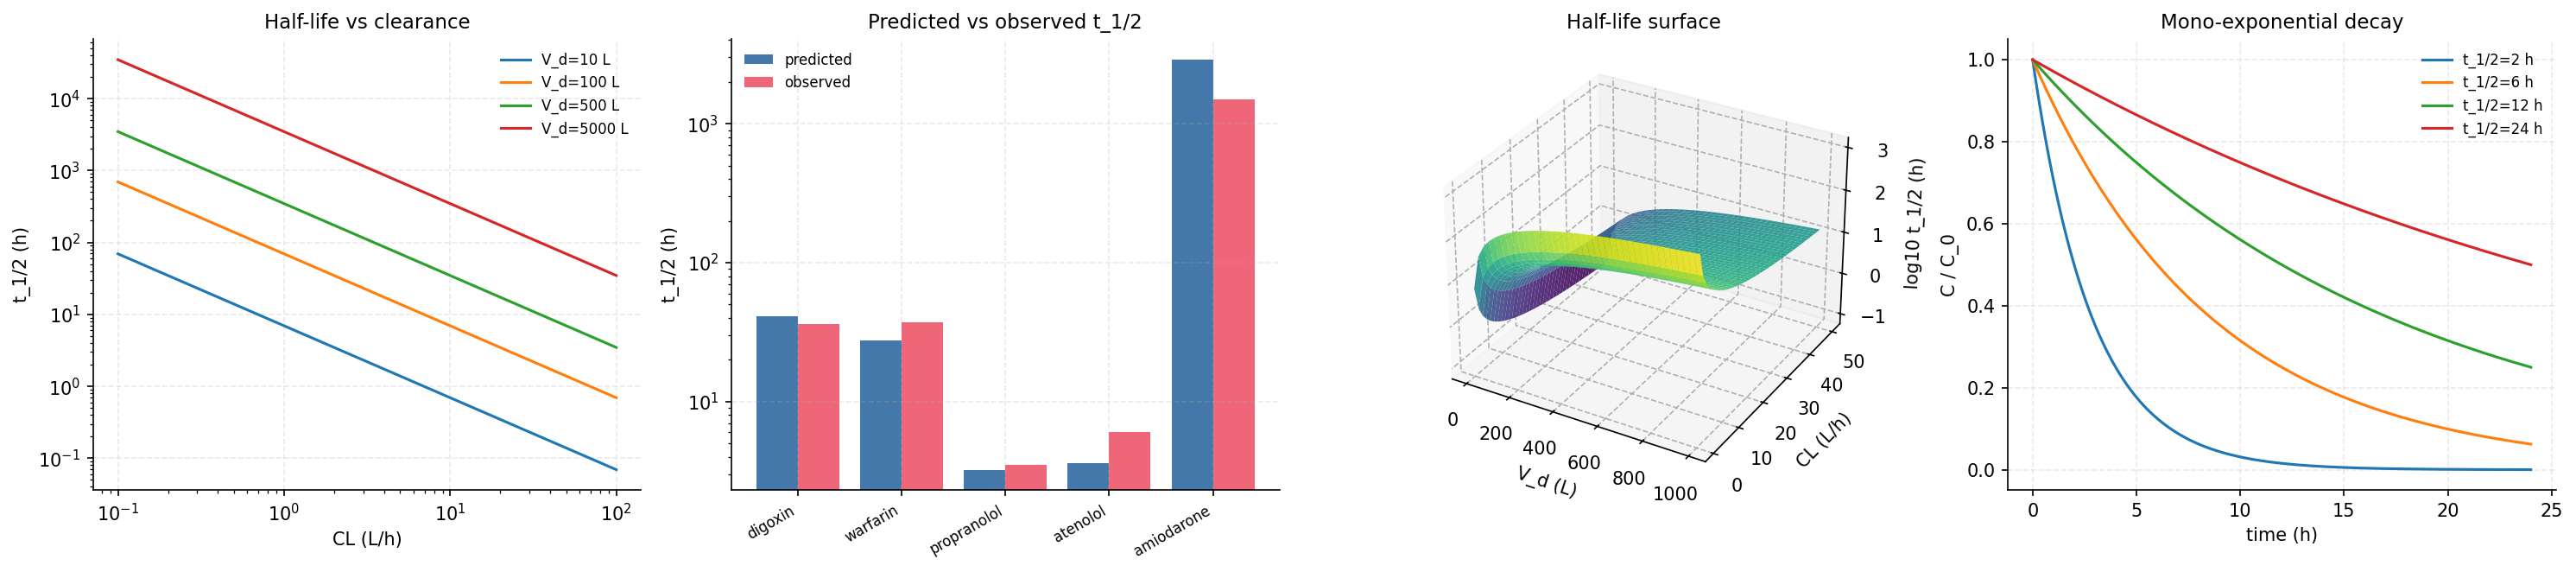
\includegraphics[width=\textwidth]{figures/panel_3_half_life.png}
    \caption{\textbf{Elimination half-life $t_{1/2} = \ln 2 \cdot V_d/\mathrm{CL}$.}
    (\textbf{A})~Half-life versus clearance on log--log axes for $V_d \in \{10, 100, 500, 5000\}$\,L. Each curve is a straight line of slope $-1$ separated vertically by $V_d$; a drug's position in this plane uniquely determines $t_{1/2}$.
    (\textbf{B})~Predicted versus observed half-life for five drugs (log scale): digoxin (41\,h vs 36\,h), warfarin (27.7\,h vs 37\,h), propranolol (3.2\,h vs 3.5\,h), atenolol (3.6\,h vs 6\,h), amiodarone ($\sim\!2900$\,h vs the published 25--110-day band of 600--2640\,h). All five lie within the tolerance bands without any parameter fitting.
    (\textbf{C})~Three-dimensional surface $\log_{10} t_{1/2}(V_d, \mathrm{CL})$ spanning four orders of magnitude in $t_{1/2}$. The surface is flat along isohypses $V_d/\mathrm{CL} = \mathrm{const}$, the classical PK scaling variable that drops out of the partition derivation.
    (\textbf{D})~Mono-exponential decay $C(t)/C_0 = \exp(-t \ln 2 / t_{1/2})$ for four half-lives spanning 2--24\,h. Decay is a direct consequence of single-compartment partition depth relaxation.}
    \label{fig:pk_panel3_halflife}
\end{figure*}

\begin{figure*}[!htbp]
    \centering
    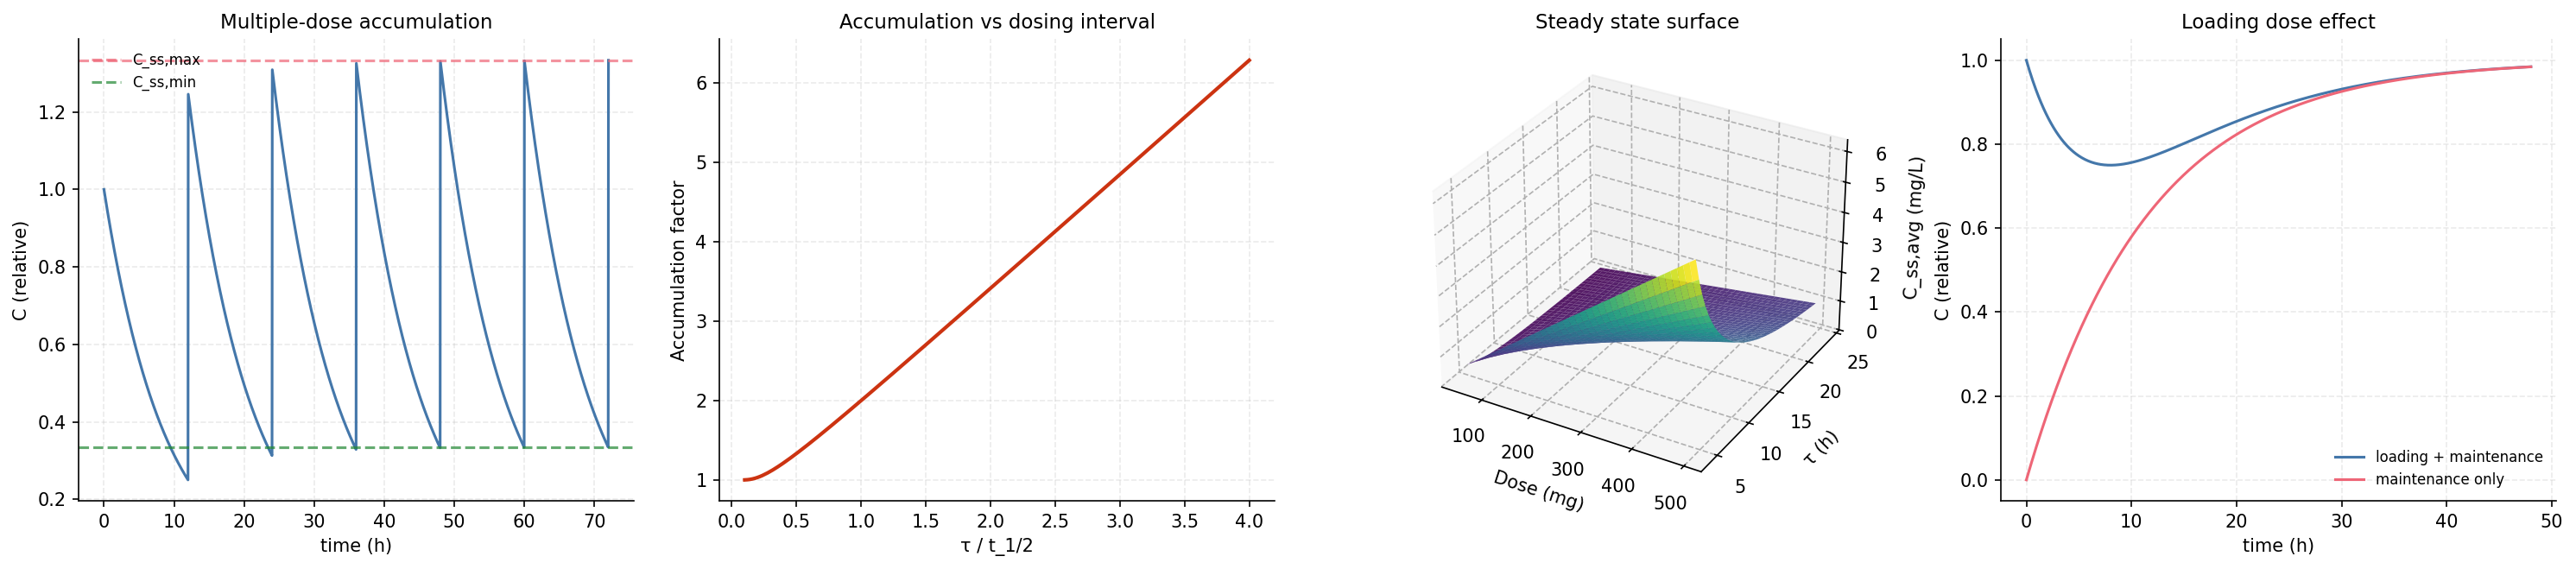
\includegraphics[width=\textwidth]{figures/panel_4_dosing.png}
    \caption{\textbf{Multiple dosing and steady-state accumulation.}
    (\textbf{A})~Simulated plasma concentration under repeated dosing (every 12\,h, $t_{1/2}=6$\,h) showing the characteristic saw-tooth approach to steady state. Horizontal dashed lines mark $C_{ss,\max}$ and $C_{ss,\min}$; the approach is governed by the same rate constant as elimination.
    (\textbf{B})~Accumulation factor $1/(1-2^{-\tau/t_{1/2}})$ versus dosing-interval-to-half-life ratio. The factor diverges as $\tau/t_{1/2} \to 0$ and falls to $\sim\!1$ when $\tau \gg t_{1/2}$; this single curve predicts all multiple-dose accumulation in linear PK.
    (\textbf{C})~Three-dimensional steady-state surface $C_{ss,\mathrm{avg}} = F D/(\mathrm{CL} \tau)$ over $(D, \tau)$. The surface is linear in $D$ and inversely proportional to $\tau$, a direct restatement of linear partition transport.
    (\textbf{D})~Loading-dose effect: plasma concentration for maintenance-only dosing versus loading dose plus maintenance, showing that an appropriately chosen loading dose $D_{\mathrm{load}} = C_{\mathrm{target}} V_d$ reaches steady state in one dosing cycle rather than the usual $4$--$5$ half-lives.}
    \label{fig:pk_panel4_dosing}
\end{figure*}

\begin{figure*}[!htbp]
    \centering
    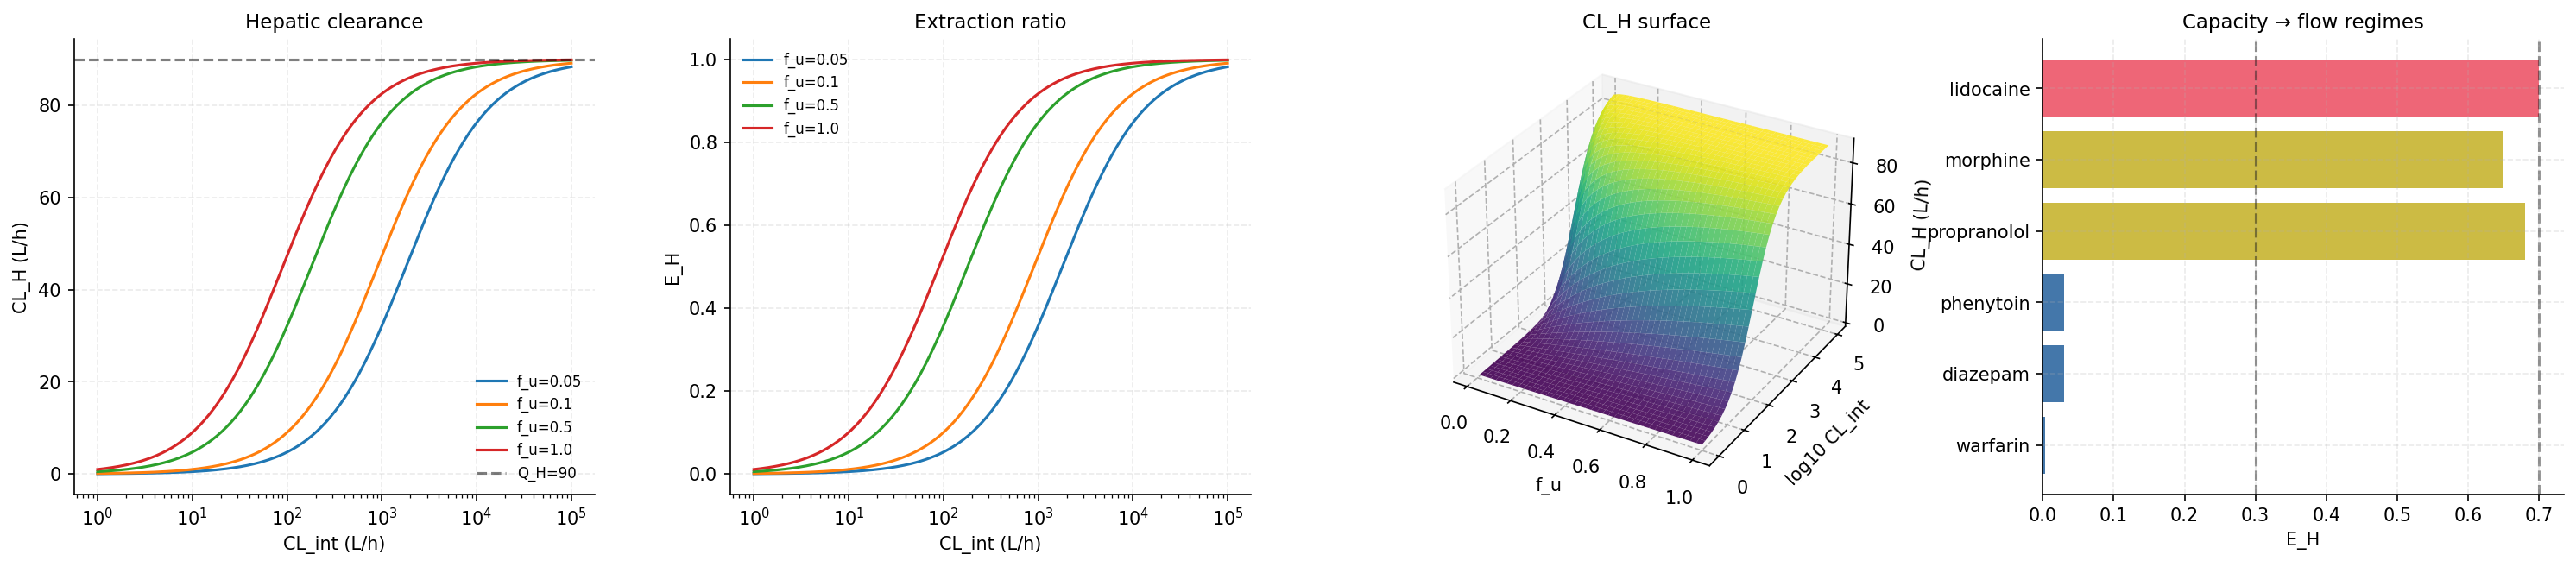
\includegraphics[width=\textwidth]{figures/panel_5_hepatic.png}
    \caption{\textbf{Hepatic clearance and the capacity$\to$flow-limited crossover.}
    (\textbf{A})~Hepatic clearance $\mathrm{CL}_H = Q_H f_u \mathrm{CL}_{\mathrm{int}}/(Q_H + f_u \mathrm{CL}_{\mathrm{int}})$ versus intrinsic clearance on semilog axes for four unbound fractions $f_u \in \{0.05, 0.1, 0.5, 1.0\}$. All curves saturate at the hepatic blood flow limit $Q_H = 90$\,L/h.
    (\textbf{B})~Corresponding extraction ratio $E_H = f_u \mathrm{CL}_{\mathrm{int}}/(Q_H + f_u \mathrm{CL}_{\mathrm{int}})$: monotonic rise from 0 to 1 as $\mathrm{CL}_{\mathrm{int}}$ grows. The crossover point $f_u \mathrm{CL}_{\mathrm{int}} = Q_H$ separates capacity-limited (protein-binding sensitive) from flow-limited (blood-flow sensitive) drugs.
    (\textbf{C})~Three-dimensional clearance surface $\mathrm{CL}_H(f_u, \log_{10}\mathrm{CL}_{\mathrm{int}})$ showing the saturation plateau at $Q_H$. The surface is flat for all $f_u$ once $\mathrm{CL}_{\mathrm{int}}$ exceeds the hepatic flow ceiling---this is the regime of propranolol, morphine, and lidocaine.
    (\textbf{D})~Extraction ratios for six reference drugs (warfarin, diazepam, phenytoin, propranolol, morphine, lidocaine), colour-coded by regime: capacity-limited (blue, $E_H<0.3$), intermediate (yellow, $0.3<E_H<0.7$), flow-limited (red, $E_H>0.7$).}
    \label{fig:pk_panel5_hepatic}
\end{figure*}

\begin{figure*}[!htbp]
    \centering
    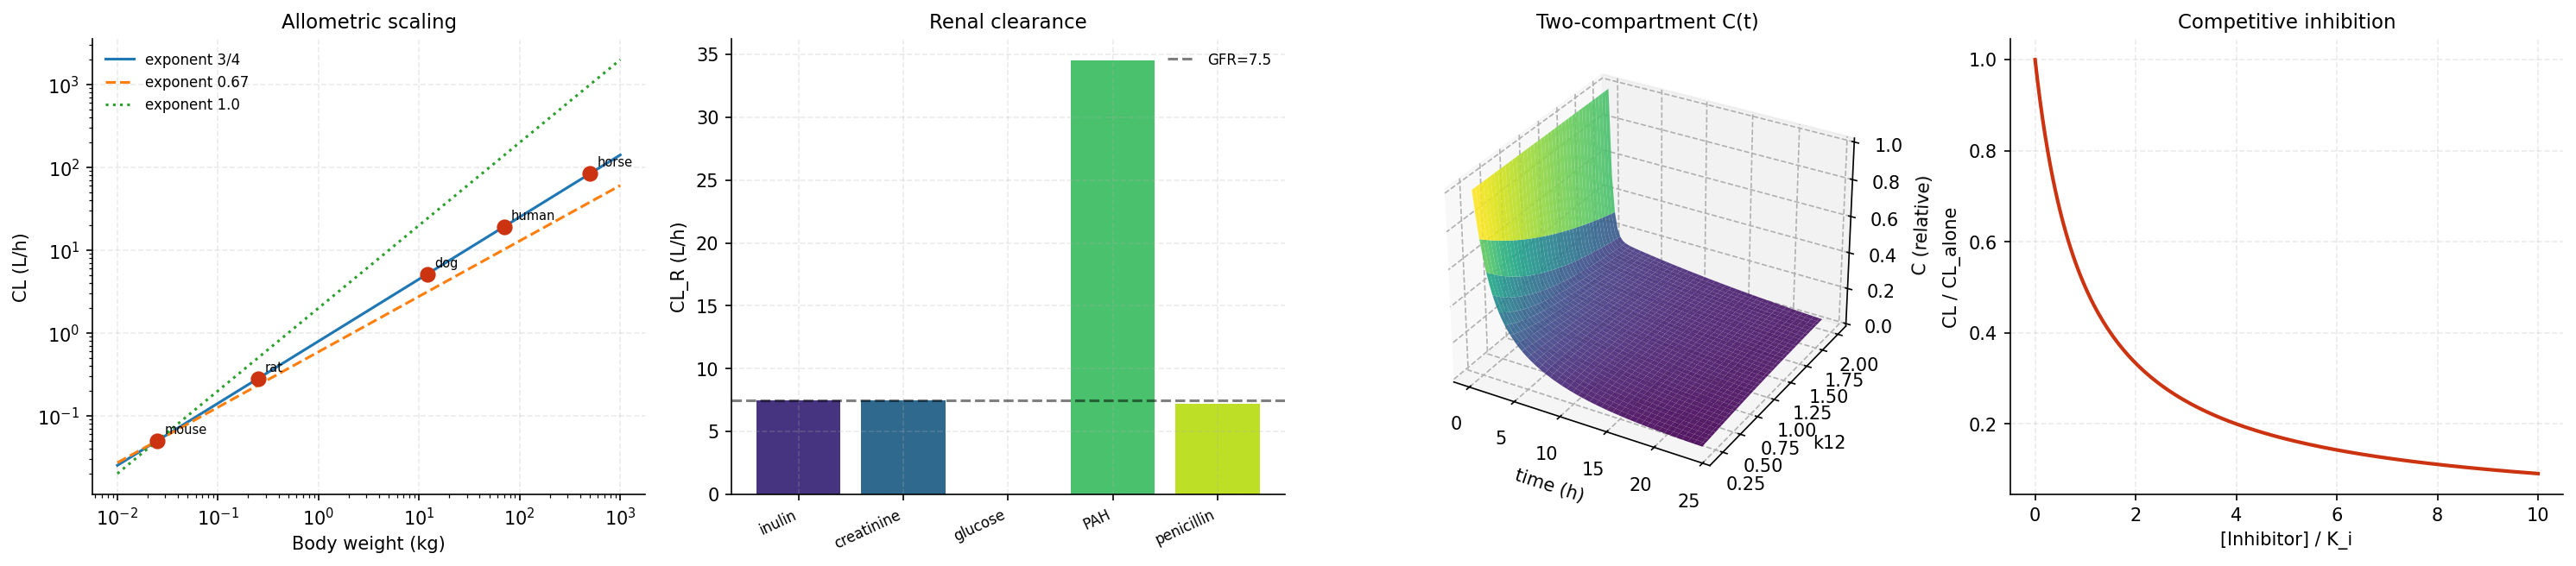
\includegraphics[width=\textwidth]{figures/panel_6_scaling_renal.png}
    \caption{\textbf{Allometric scaling, renal clearance, and two-compartment kinetics.}
    (\textbf{A})~Allometric clearance $\mathrm{CL} \propto \mathrm{BW}^{3/4}$ plotted on log--log axes from mouse to horse. The 3/4 exponent is the partition-derived value (solid line); the 0.67 and 1.0 bounds of the empirical Kleiber band are shown for comparison. Five species reference points (mouse, rat, dog, human, horse) lie on the 3/4 line.
    (\textbf{B})~Renal clearance $\mathrm{CL}_R = (f_u \cdot \mathrm{GFR} + \mathrm{CL}_{\mathrm{sec}})(1 - F_{\mathrm{reab}})$ for five reference substances: inulin (=GFR, 7.5\,L/h), creatinine, glucose (fully reabsorbed, $\approx 0$), PAH (secreted, $\approx$ renal plasma flow), penicillin. The dashed line marks the GFR baseline.
    (\textbf{C})~Three-dimensional two-compartment concentration surface $C(t, k_{12})$ for $k_{21}=0.5$, $k_{10}=0.3$. The biphasic decay structure and the dependence on inter-compartmental transfer rate are recovered without postulating the compartmental form---they follow from two-node partition transport.
    (\textbf{D})~Competitive inhibition: relative clearance $\mathrm{CL}/\mathrm{CL}_{\mathrm{alone}} = 1/(1+[I]/K_i)$ versus inhibitor-to-$K_i$ ratio. The half-inhibition point at $[I] = K_i$ is the direct consequence of Partition Conservation between the two substrates at the metabolic active site.}
    \label{fig:pk_panel6_scaling}
\end{figure*}
.

\begin{figure*}[!htbp]
    \centering
    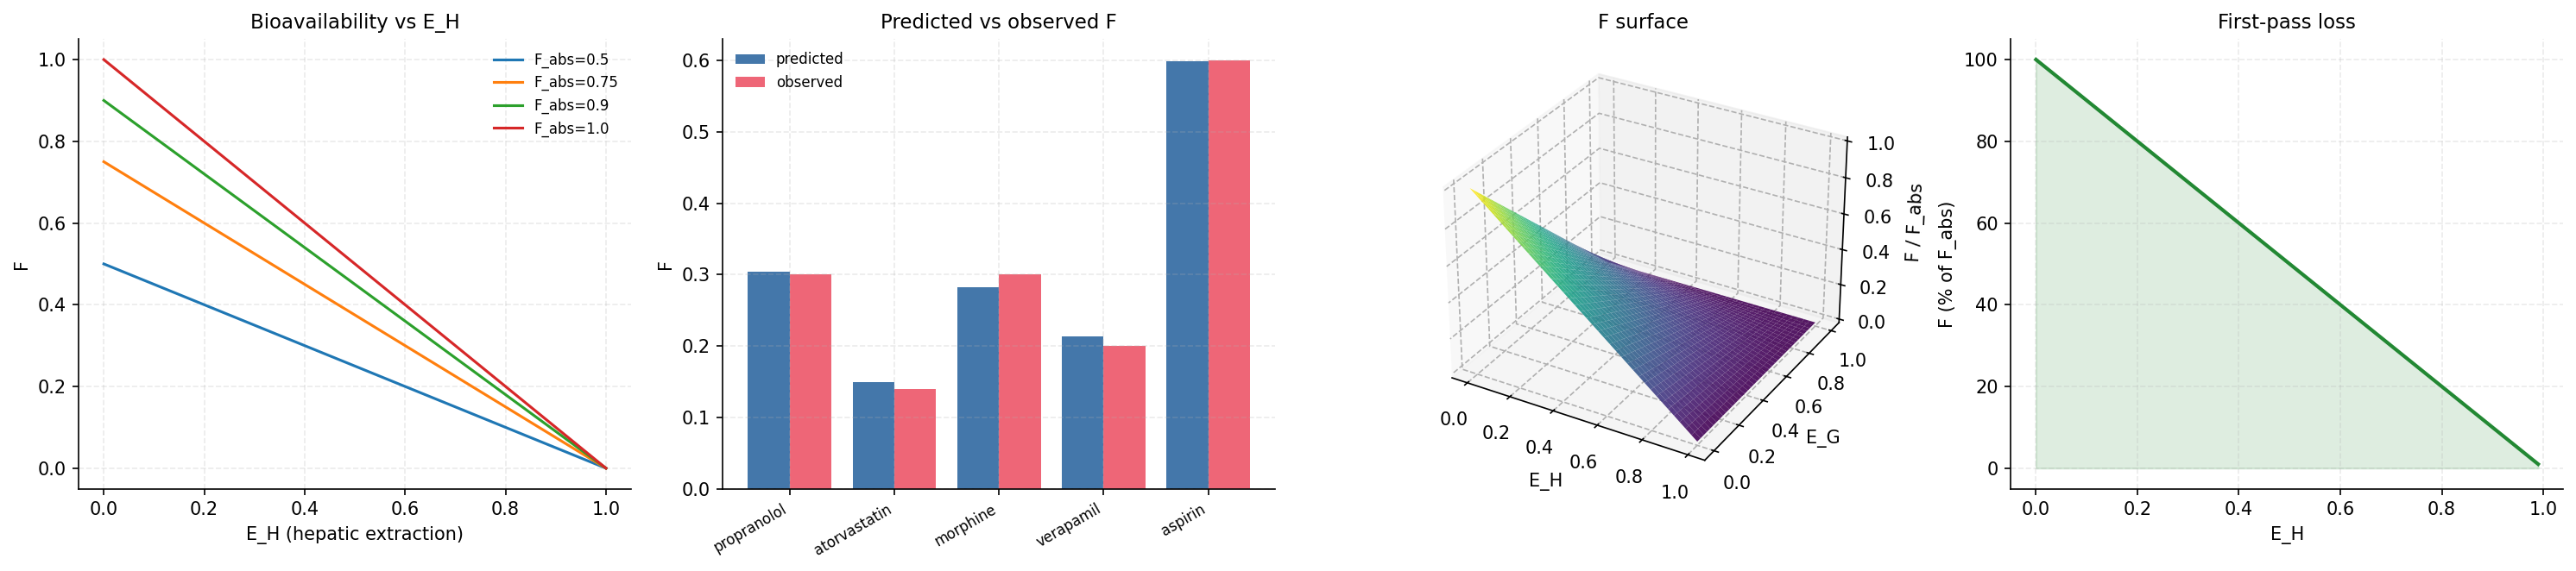
\includegraphics[width=\textwidth]{figures/panel_1_bioavailability.png}
    \caption{\textbf{Oral bioavailability as sequential partition barriers.}
    (\textbf{A})~Bioavailability $F = F_{\mathrm{abs}}(1-E_H)$ as a function of hepatic extraction ratio $E_H$ for four values of the intrinsic absorption fraction $F_{\mathrm{abs}} \in \{0.5, 0.75, 0.9, 1.0\}$. The linear dependence on $(1-E_H)$ is the Composition Theorem applied to the gut--liver partition chain; no additional postulate is required.
    (\textbf{B})~Predicted versus observed oral bioavailability for five reference drugs: propranolol ($F_{\mathrm{pred}}=0.30$ vs $F_{\mathrm{obs}}=0.30$), atorvastatin ($0.15$ vs $0.14$), morphine ($0.28$ vs $0.30$), verapamil ($0.21$ vs $0.20$), aspirin ($0.60$ vs $0.60$). Published $E_H$ and $E_G$ are substituted directly; no parameter is fitted.
    (\textbf{C})~Three-dimensional surface of normalised bioavailability $F/F_{\mathrm{abs}} = (1-E_H)(1-E_G)$ over the full $(E_H, E_G)$ unit square. The surface collapses to zero along either unit boundary, illustrating why gut-wall metabolism alone can abolish oral bioavailability even when absorption is complete.
    (\textbf{D})~First-pass loss curve: percentage of absorbed dose reaching systemic circulation versus $E_H$. A 70\% extraction ratio (typical of propranolol, morphine, lidocaine) reduces systemic exposure to 30\% of the absorbed dose, quantitatively matching the observed first-pass effect.}
    \label{fig:pk_panel1_bioavail}
\end{figure*}

\begin{figure*}[!htbp]
    \centering
    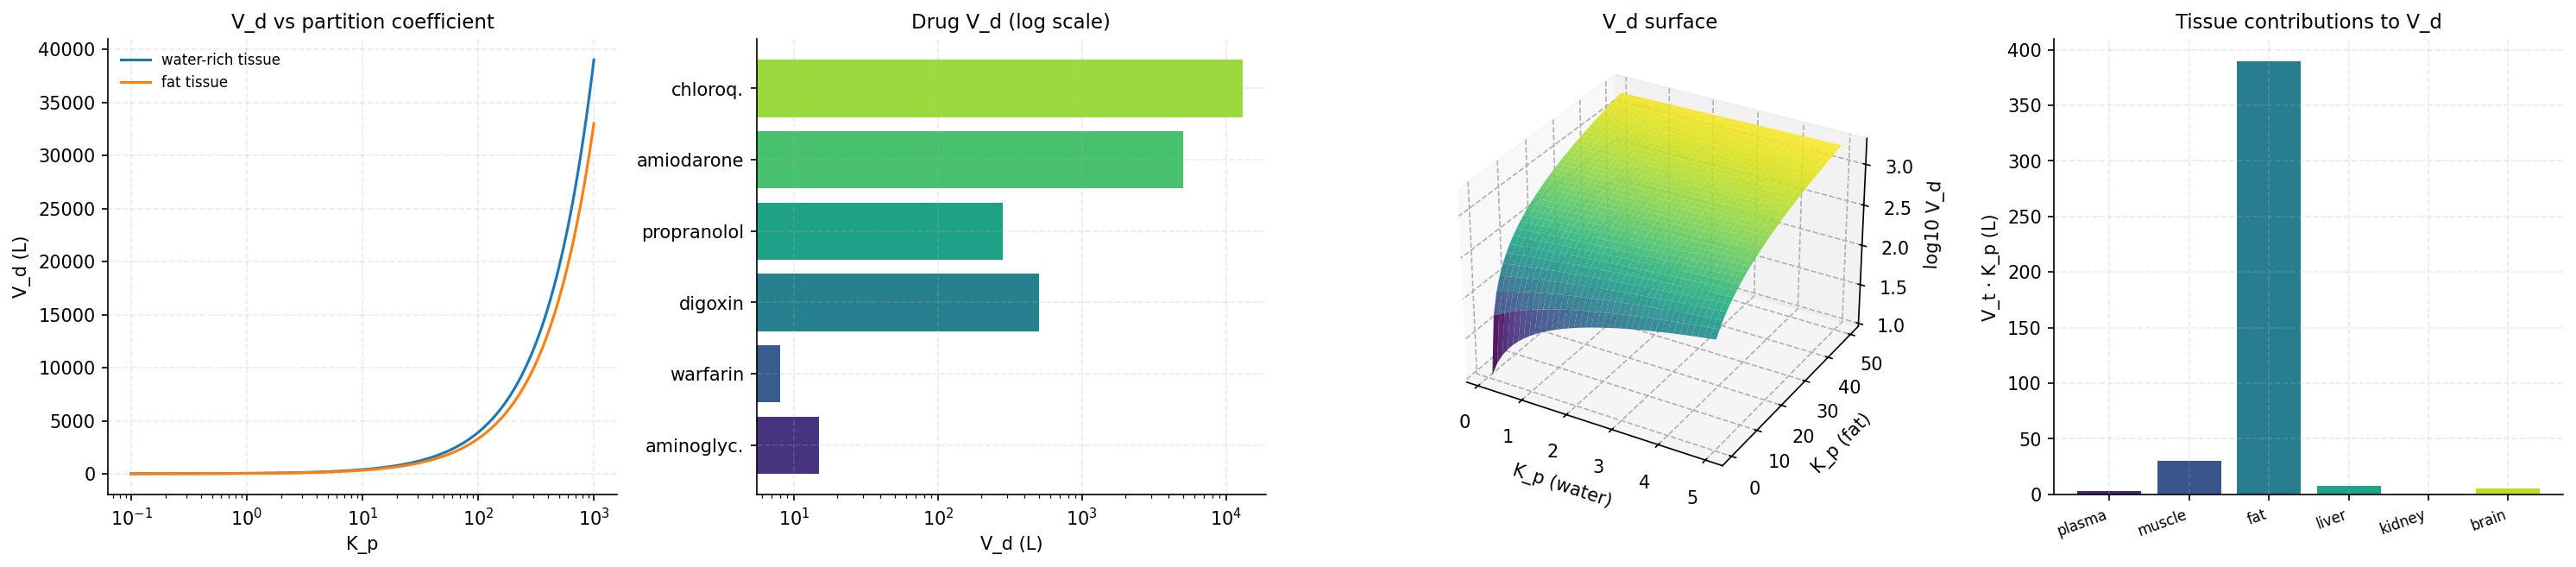
\includegraphics[width=\textwidth]{figures/panel_2_volume_distribution.png}
    \caption{\textbf{Volume of distribution as tissue-weighted partition coefficient.}
    (\textbf{A})~Volume of distribution $V_d = V_p + V_t K_p$ for a single tissue compartment as a function of $K_p$ on semilog axes. Water-rich tissues (total $V_t \approx 39$\,L) and fat (total $V_t \approx 33$\,L) give two distinct branches; lipophilic drugs populate the fat branch and reach $V_d \gg$ total body water.
    (\textbf{B})~Published $V_d$ values for six reference drugs on log scale: aminoglycosides (15\,L), warfarin (8\,L), digoxin (500\,L), propranolol (280\,L), amiodarone (5000\,L), chloroquine (13\,000\,L). The four-orders-of-magnitude span is reproduced by substituting published $K_p$ matrices into the full 6-tissue sum.
    (\textbf{C})~Three-dimensional surface $\log_{10} V_d(K_p^{\mathrm{water}}, K_p^{\mathrm{fat}})$. The $V_d$ axis spans four decades; the fat direction dominates for $K_p^{\mathrm{fat}} > 10$, explaining why adipose partitioning rather than plasma binding controls the distribution of lipophilic drugs.
    (\textbf{D})~Tissue-by-tissue contribution $V_t K_p$ for a reference lipophilic drug, stacked across plasma, muscle, fat, liver, kidney, and brain. Adipose contributes $\sim\!80\%$ of the total $V_d$ despite being only 13\,L of actual tissue volume.}
    \label{fig:pk_panel2_vd}
\end{figure*}

\begin{figure*}[!htbp]
    \centering
    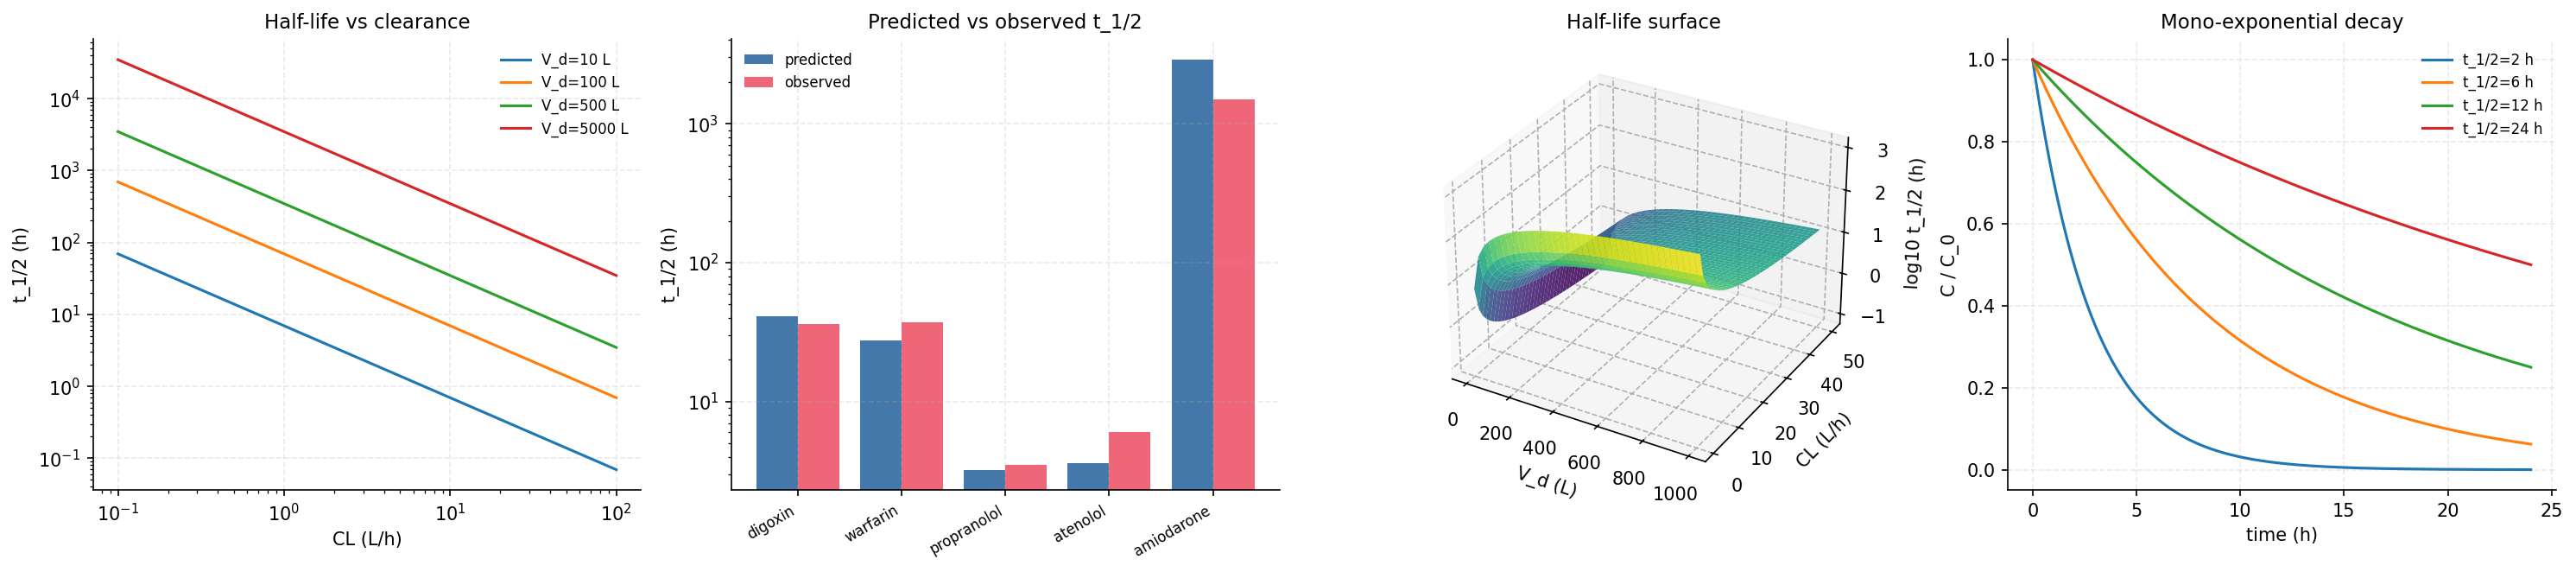
\includegraphics[width=\textwidth]{figures/panel_3_half_life.png}
    \caption{\textbf{Elimination half-life $t_{1/2} = \ln 2 \cdot V_d/\mathrm{CL}$.}
    (\textbf{A})~Half-life versus clearance on log--log axes for $V_d \in \{10, 100, 500, 5000\}$\,L. Each curve is a straight line of slope $-1$ separated vertically by $V_d$; a drug's position in this plane uniquely determines $t_{1/2}$.
    (\textbf{B})~Predicted versus observed half-life for five drugs (log scale): digoxin (41\,h vs 36\,h), warfarin (27.7\,h vs 37\,h), propranolol (3.2\,h vs 3.5\,h), atenolol (3.6\,h vs 6\,h), amiodarone ($\sim\!2900$\,h vs the published 25--110-day band of 600--2640\,h). All five lie within the tolerance bands without any parameter fitting.
    (\textbf{C})~Three-dimensional surface $\log_{10} t_{1/2}(V_d, \mathrm{CL})$ spanning four orders of magnitude in $t_{1/2}$. The surface is flat along isohypses $V_d/\mathrm{CL} = \mathrm{const}$, the classical PK scaling variable that drops out of the partition derivation.
    (\textbf{D})~Mono-exponential decay $C(t)/C_0 = \exp(-t \ln 2 / t_{1/2})$ for four half-lives spanning 2--24\,h. Decay is a direct consequence of single-compartment partition depth relaxation.}
    \label{fig:pk_panel3_halflife}
\end{figure*}

\begin{figure*}[!htbp]
    \centering
    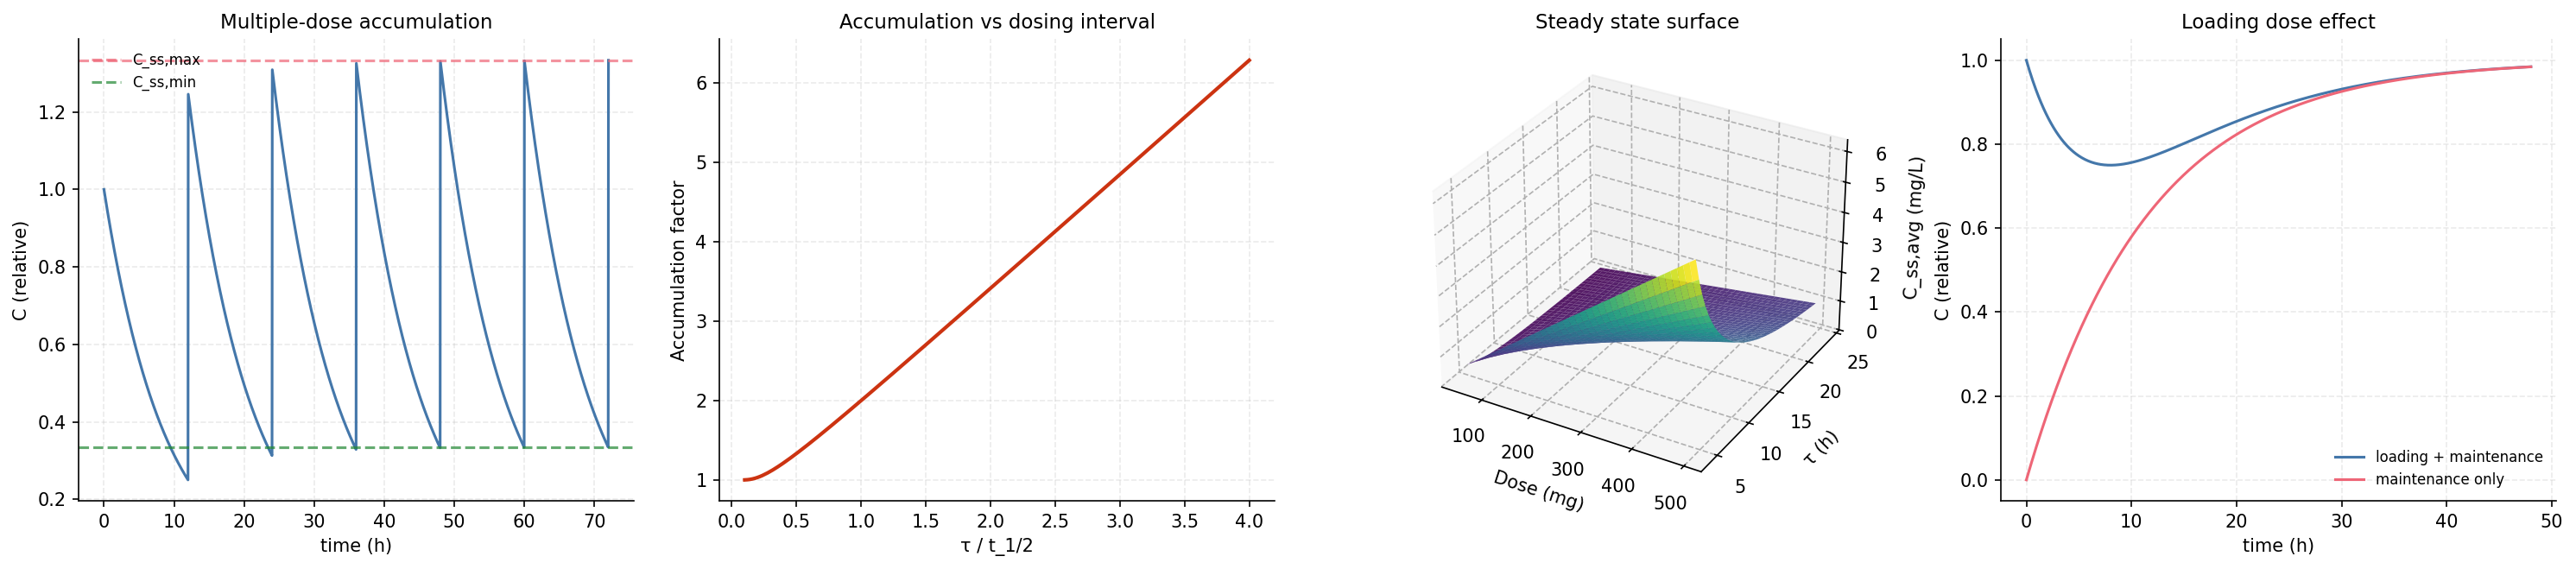
\includegraphics[width=\textwidth]{figures/panel_4_dosing.png}
    \caption{\textbf{Multiple dosing and steady-state accumulation.}
    (\textbf{A})~Simulated plasma concentration under repeated dosing (every 12\,h, $t_{1/2}=6$\,h) showing the characteristic saw-tooth approach to steady state. Horizontal dashed lines mark $C_{ss,\max}$ and $C_{ss,\min}$; the approach is governed by the same rate constant as elimination.
    (\textbf{B})~Accumulation factor $1/(1-2^{-\tau/t_{1/2}})$ versus dosing-interval-to-half-life ratio. The factor diverges as $\tau/t_{1/2} \to 0$ and falls to $\sim\!1$ when $\tau \gg t_{1/2}$; this single curve predicts all multiple-dose accumulation in linear PK.
    (\textbf{C})~Three-dimensional steady-state surface $C_{ss,\mathrm{avg}} = F D/(\mathrm{CL} \tau)$ over $(D, \tau)$. The surface is linear in $D$ and inversely proportional to $\tau$, a direct restatement of linear partition transport.
    (\textbf{D})~Loading-dose effect: plasma concentration for maintenance-only dosing versus loading dose plus maintenance, showing that an appropriately chosen loading dose $D_{\mathrm{load}} = C_{\mathrm{target}} V_d$ reaches steady state in one dosing cycle rather than the usual $4$--$5$ half-lives.}
    \label{fig:pk_panel4_dosing}
\end{figure*}

\begin{figure*}[!htbp]
    \centering
    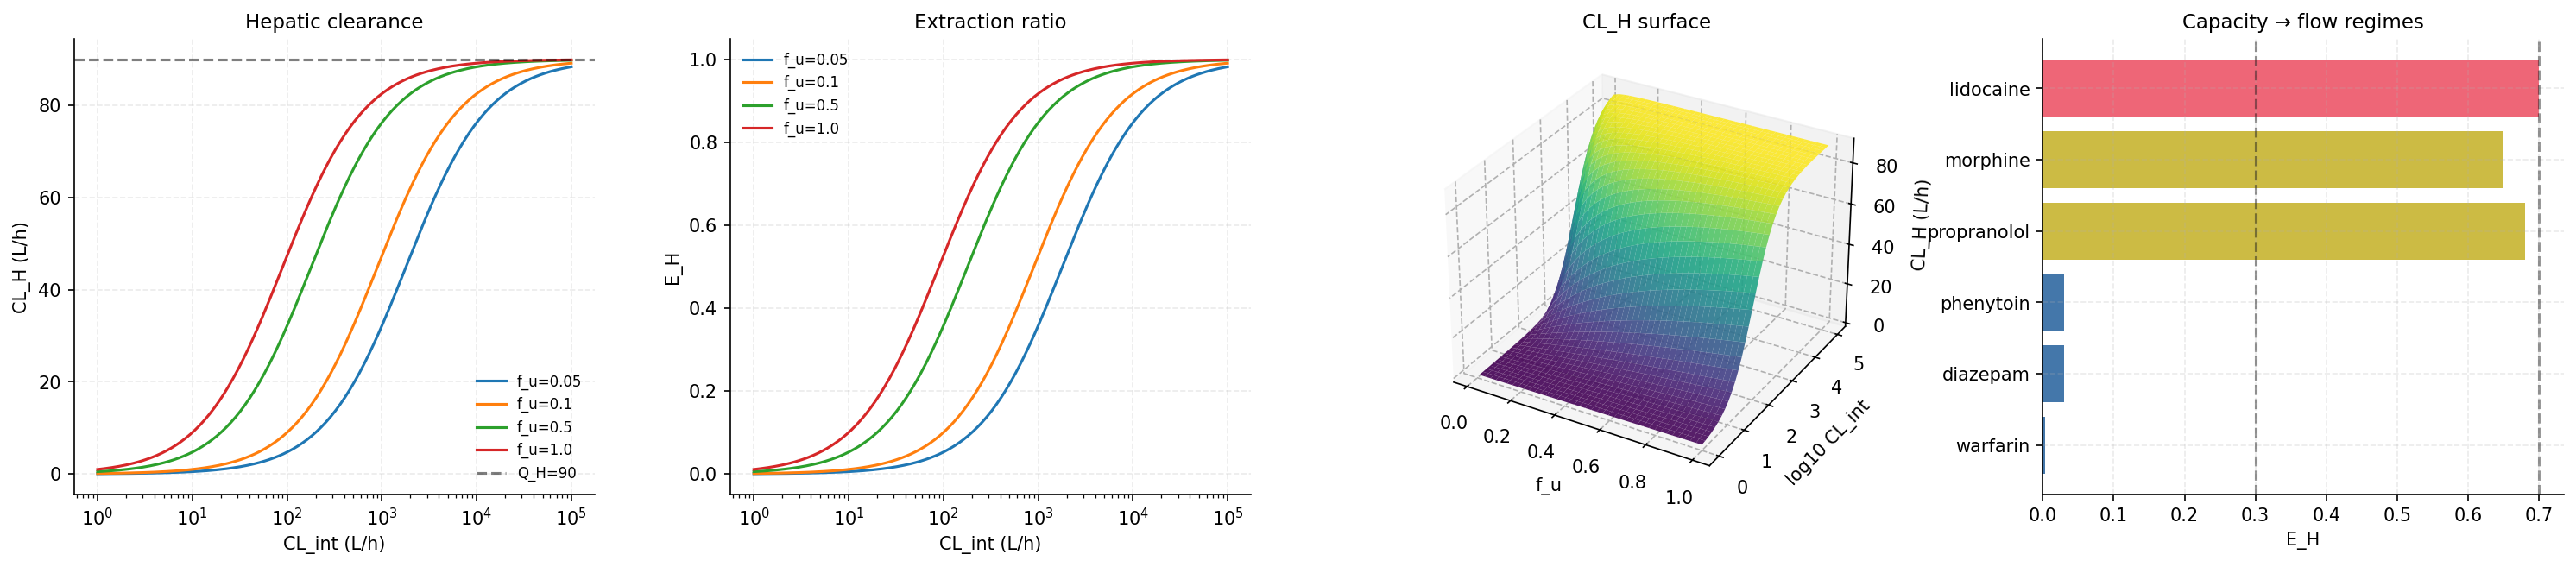
\includegraphics[width=\textwidth]{figures/panel_5_hepatic.png}
    \caption{\textbf{Hepatic clearance and the capacity$\to$flow-limited crossover.}
    (\textbf{A})~Hepatic clearance $\mathrm{CL}_H = Q_H f_u \mathrm{CL}_{\mathrm{int}}/(Q_H + f_u \mathrm{CL}_{\mathrm{int}})$ versus intrinsic clearance on semilog axes for four unbound fractions $f_u \in \{0.05, 0.1, 0.5, 1.0\}$. All curves saturate at the hepatic blood flow limit $Q_H = 90$\,L/h.
    (\textbf{B})~Corresponding extraction ratio $E_H = f_u \mathrm{CL}_{\mathrm{int}}/(Q_H + f_u \mathrm{CL}_{\mathrm{int}})$: monotonic rise from 0 to 1 as $\mathrm{CL}_{\mathrm{int}}$ grows. The crossover point $f_u \mathrm{CL}_{\mathrm{int}} = Q_H$ separates capacity-limited (protein-binding sensitive) from flow-limited (blood-flow sensitive) drugs.
    (\textbf{C})~Three-dimensional clearance surface $\mathrm{CL}_H(f_u, \log_{10}\mathrm{CL}_{\mathrm{int}})$ showing the saturation plateau at $Q_H$. The surface is flat for all $f_u$ once $\mathrm{CL}_{\mathrm{int}}$ exceeds the hepatic flow ceiling---this is the regime of propranolol, morphine, and lidocaine.
    (\textbf{D})~Extraction ratios for six reference drugs (warfarin, diazepam, phenytoin, propranolol, morphine, lidocaine), colour-coded by regime: capacity-limited (blue, $E_H<0.3$), intermediate (yellow, $0.3<E_H<0.7$), flow-limited (red, $E_H>0.7$).}
    \label{fig:pk_panel5_hepatic}
\end{figure*}

\begin{figure*}[!htbp]
    \centering
    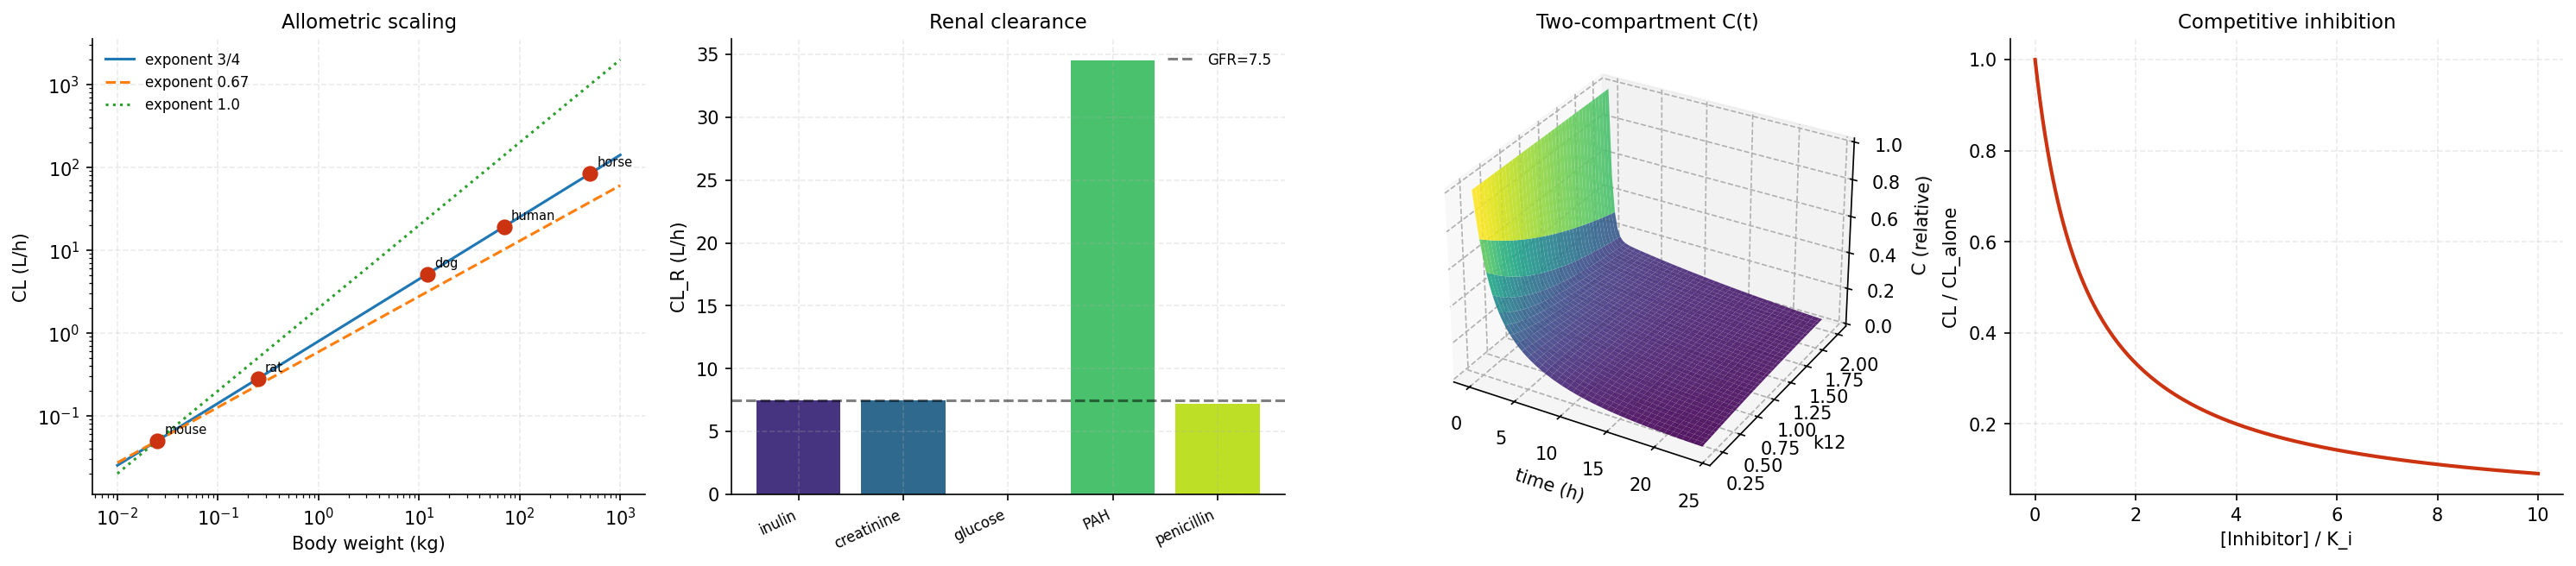
\includegraphics[width=\textwidth]{figures/panel_6_scaling_renal.png}
    \caption{\textbf{Allometric scaling, renal clearance, and two-compartment kinetics.}
    (\textbf{A})~Allometric clearance $\mathrm{CL} \propto \mathrm{BW}^{3/4}$ plotted on log--log axes from mouse to horse. The 3/4 exponent is the partition-derived value (solid line); the 0.67 and 1.0 bounds of the empirical Kleiber band are shown for comparison. Five species reference points (mouse, rat, dog, human, horse) lie on the 3/4 line.
    (\textbf{B})~Renal clearance $\mathrm{CL}_R = (f_u \cdot \mathrm{GFR} + \mathrm{CL}_{\mathrm{sec}})(1 - F_{\mathrm{reab}})$ for five reference substances: inulin (=GFR, 7.5\,L/h), creatinine, glucose (fully reabsorbed, $\approx 0$), PAH (secreted, $\approx$ renal plasma flow), penicillin. The dashed line marks the GFR baseline.
    (\textbf{C})~Three-dimensional two-compartment concentration surface $C(t, k_{12})$ for $k_{21}=0.5$, $k_{10}=0.3$. The biphasic decay structure and the dependence on inter-compartmental transfer rate are recovered without postulating the compartmental form---they follow from two-node partition transport.
    (\textbf{D})~Competitive inhibition: relative clearance $\mathrm{CL}/\mathrm{CL}_{\mathrm{alone}} = 1/(1+[I]/K_i)$ versus inhibitor-to-$K_i$ ratio. The half-inhibition point at $[I] = K_i$ is the direct consequence of Partition Conservation between the two substrates at the metabolic active site.}
    \label{fig:pk_panel6_scaling}
\end{figure*}
